\documentclass[twoside]{AiTeX}
\usepackage{flafter}


\title{Memoria DSI}
\author{Grupo 2}
\date{Octubre 2023}
\begin{document}
%\datos{facultad}{universidad}{grado}{asignatura}{subtitulo}{autor}{curso}
\datos{Informática}{Universidad Complutense de Madrid}{Ingeniería informática}{Just Travel It}{Memoria de proyecto - Hito 2}{ \underline{\textbf{Grupo 2}} \\ Alejandro Barrachina Argudo \\
Sergio Colet García\\
Maria Esteban Benito \\
Javier Gómez Arribas \\
Leire Jiménez González \\
Pablo Lavandeira Poyato \\
Laura Martínez Tomás \\
Guillermo Novillo Díaz \\
Rodrigo Souto Santos \\
Carlos Varela Sansano \\
Daniel Yllana Santiago
}{2023-2024}
\portadaApuntes
\pagestyle{empty}
\tableofcontents 
\pagestyle{empty}
\justify
\pagestyle{fancy}

\newpage

\newacronym{di}{D.I.}{Discapacidad Intelectual}


% \section*{Control de cambios} %
% \noindent\begin{tabularx}{\textwidth}{ |l|l|p{5cm}|X| }
%     \hline
%     \textbf{Versión} & \textbf{Fecha} & \textbf{Autores}     & \textbf{Descripción}                                                 \\
%     \hline
%     1.0              & 27/09/2023     & Alejandro Barrachina & Comienzo de la memoria\\
%     \hline
% \end{tabularx}

% \newpage

\chapterA{Hito 2: Fase de Modelado}
\section{Listado de factoides}
El listado de factoides es el producto resultado de la fase de investigación. Para obtenerlo se ha extraído las principales características de las
diversas entrevistas, de todas las respuestas a los cuestionarios y del análisis de la competencia. Respecto a los obtenidos en el anterior hito,
hemos realizado una serie de cambios debido a la falta de respuestas a algunas de las variables que hemos identificado y a los problemas que se
han podido identificar durante la corrección de dichos factoides.


Tras la corrección del hito anterior y observando las necesidades del diseño de personas de este hito, vamos a realizar una serie de modificaciones
en la lista de factoides, reflejando los cambios que han sido realizados con la letra en cursiva. Cabe destacar que el usuario Alberto ha sido finalmente
descartado debido a que sus características no se encuadraban dentro de las propuestas en la hipótesis de usuarios. \\

\textbf{Factoides de Madi:}

\begin{itemize}
    \item Madi es secretaria de la FEDDI y lleva 16 años trabajando allí.
    \item Madi se encarga de organizar los viajes cuadrando horarios y comprando billetes.
    \item Madi compra billetes a través de Renfe, Air Europa o Iberia porque le sale más económico que en un comparador.
    \item Madi se encarga de los viajes de campeonatos internacionales que les recepciona, les recoge y les lleva al punto de encuentro.
    \item Madi ve que el problema principal para los deportistas es la dependencia de sus padres y entrenadores, el manejo de las aplicaciones y el internet y para algunos necesitan acompañante.
    \item Madi considera que necesitan acompañantes porque tienen problemas para orientarse y no se manejan bien.
    \item Para Madi las dificultades dependen mucho del grado de discapacidad.
    \item Madi no usa aplicaciones, sólo compra en páginas oficiales de la aerolínea.
    \item Madi utiliza la agencia de viajes Betravel para vuelos internacionales.
    \item Madi descarta Ryanair.
    \item Madi no utiliza comparadores porque ya tiene localizadas dos compañías y Renfe que ofrecen el servicio de acompañamiento de AENA.
    \item Madi tiene en cuenta el precio y la variedad de horarios para coger un billete.
    \item Madi no se fija en más facilidades, esos son los atletas.
    \item Madi considera que el comparador debe ser muy simple (lugar, destino y fecha).
    \item A Madi le parece importante que se pueda ver qué tipos de servicios de acompañantes ofrecen.
    \item \textit{En los campeonatos de España son los clubes los encargados del desplazamiento de los deportistas (ella no interviene)}.
\end{itemize}


\textbf{Factoides de Sofia:}

\begin{itemize}
    \item \textit{Sofía es estudiante, tiene 21 años y considera que tiene un buen manejo de la tecnología.}
    \item \textit{A Sofia le gusta viajar y considera que es uno de sus hobbies favoritos porque le gusta conocer nuevas culturas, vivir experiencias y explorar lugares desconocidos.}
    \item \textit{Sofía ha viajado por Europa, Estados Unidos y por el territorio nacional.}
    \item \textit{A Sofia le gustaría viajar más.}
    \item \textit{Sofía usa distintos métodos de transporte como coche, transporte público, avión, tren, bus y privado, este último rara vez.}
    \item \textit{Sofía prefiere usar autobuses solo cuando viaje distancias cortas o medias.}
    \item \textit{Sofía normalmente suele viajar con amigos y familiares por ocio.}
    \item \textit{Sofía no recuerda haber tenido ningún problema viajando, aunque admite que cuando viaja lo hace con la mente más abierta de lo que la tiene normalmente.}
    \item \textit{Sofía a veces organiza los viajes que hace y a veces no.}
    \item \textit{Sofía busca viajes económicos y que se adapten a sus necesidades.}
    \item \textit{Sofia utiliza varios comparadores de viajes a la hora de organizar un viaje para buscar las mejores ofertas. Por ejemplo: Kayak, Skyscanner, Trivago.}
    \item \textit{A Sofía le gustaría que los comparadores de viajes mostraran el precio final del billete, con los posibles extras incluidos, piensa que es un punto a mejorar.}
    \item \textit{Sofía prefiere usar aplicaciones web a aplicaciones móviles, y suele hacer estas gestiones desde el ordenador.}
    \item \textit{Sofía piensa que algunos comparadores son tediosos a la hora de usar ya que algunos tardan mucho en cargar o te redirigen a otra páginas.}
    \item \textit{Cuando Sofía ha tenido problemas con algún comparador ha optado por usar otro comparador que no tuviera esos problemas.}
    \item \textit{Sofía considera que con una interfaz sencilla y fácil de usar sería suficiente para un comparador.}
    \item \textit{Sofía considera que los comparadores de viajes son bastante accesibles, pero que quizás aclarar algunas cosas en las webs o los anuncios de spam en las webs pueden molestar a personas con discapacidad intelectual.}
    
\end{itemize}

\textbf{Factoides de Beatriz:}
\begin{itemize}
    \item Beatriz tiene 21 años.
    \item Beatriz se desenvuelve bien con las tecnologías y declara usarlas a diario.
    \item \textit{Beatriz viaja por ocio, para conocer nuevos lugares y culturas o visitar familiares.}
    \item Beatriz viaja una vez al año, sobre todo dentro de España, y fuera de España una vez cada dos años.
    \item \textit{A Beatriz le gustaría viajar más porque viaja poco para su gusto y salir de España más de una vez al año, los motivos por los que no puede hacerlo con más frecuencia es por su situación económica y el escaso tiempo que tiene de vacaciones.}
    \item Suele viajar en coche o en avión para distancias más largas.
    \item Beatriz suele viajar para visitar a familiares o por razones de ocio.
    \item Beatriz suele viajar acompañada (normalmente de sus familiares).
    \item Cuando viaja con su familia, organizan el viaje conjuntamente.
    \item \textit{Beatriz prioriza el precio del billete.}
    \item Cuando no viaja con su familia, Beatriz suele organizar los viajes que hace.
    \item Beatriz se fija sobretodo en el precio a la hora de tomar una decisión, por ejemplo, para comprar un vuelo.
    \item En su último viaje, Beatriz optó por usar una aplicación (eDreams) debido a que tenían un programa con prueba gratuita con el que sus vuelos le salieron más baratos.
    \item Beatriz prefiere los vuelos de ida tempranos y los de vuelta más tarde.
    \item A la hora de hacer la reserva, Beatriz cree que lo más tedioso son todas las pantallas que tienes que atravesar en las que te ofrecen todo tipo de servicios extra, alguno incluso ofreciéndose dos veces.
    \item A Beatriz también le gustaría que los comparadores pusieran un mensaje más claro en el caso de que ida y vuelta sean desde aeropuertos distintos.
    \item Google es su navegador favorito, principalmente porque lo lleva usando mucho tiempo y está acostumbrada, pero también debido a la conectividad con otros servicios en su móvil y porque considera que es lo mejor en cuanto a desarrollo web; también le gusta su estética.
    \item El comparador favorito de vuelos de Beatriz es el comparador de Google u otros.
    \item Beatriz considera que los comparadores de vuelos pueden no ser accesibles para personas que no tengan mucha soltura con las tecnologías.
    \item Beatriz considera que eDreams es muy estético, más que el comparador de Google o que otros.
    \item \textit{Para ella no es un problema sacrificar facilidades como el tipo y la cantidad de equipaje, la elección de asiento o los horarios de ida y vuelta para que el precio sea más barato}.
    \item \textit{Beatriz destaca también que al comprar en eDreams tuvo un problema con la aerolínea, lo que la llevó a tener que pasar un proceso poco accesible y con más cargos económicos.}
    \item \textit{Beatriz destaca que generalmente prefiere hacer estas reservas de viajes en el ordenador en vez de en el móvil.}
\end{itemize}


\textbf{Factoides del cuestionario:}

\begin{itemize}
    \item La mitad de los usuarios tienen entre 19 y 25 años y la otra mitad entre 26 y 65 años.
    \item La mayoría de los encuestados viven en la ciudad, pocos en pueblos.
    \item Dos tercios de los encuestados tienen un poder adquisitivo medio. Un tercio, bajo y muy pocos, alto.
    \item La mayoría de los encuestados les gusta viajar, pocos no.
    \item La mayoría de los encuestados le gusta viajar por conocer nuevos lugares y los pocos que no, es por la gente o por no parar de moverse.
    \item La mayoría de los encuestados viajan al menos una vez al año, el resto viajan al menos una vez al mes y muy poco no viajan.
    \item La mayoría de los encuestados le gustaría viajar más, el resto no.
    \item Todos los encuestados disfrutan cuando viajan.
    \item Los medios de transporte que usan los encuestados son coche propio, transporte público y aéreo.
    \item Los encuestados suelen viajar por ocio, pocos por trabajo.
    \item Las herramientas que más utilizan los encuestados son Trivago, Kayak y SkyScanner. Hay un tercio de los encuestados que no usan ninguna.
    \item Los comparadores de viajes (Trivago, Kayak, Rastreator, SkyScanner, Momondo) son de fácil uso.
    \item Un quinto de los encuestados tienen alguna discapacidad reconocida.
    \item Los encuestados con discapacidad la mayoría tienen discapacidad física y el resto es intelectual o mental.
    \item Los encuestados con discapacidad dos tercios necesitan adaptaciones para sus viajes como para sillas de ruedas.
    \item La mayoría de los encuestados con discapacidad a veces planifican y el resto o nunca o siempre.
    \item Un tercio de los encuestados con discapacidad encuentran dificultad en el proceso de búsqueda por la accesibilidad.
    \item La mayoría de los encuestados con discapacidad no les supone una dificultad buscar medio de transporte, hacer, comparar y ver las ventajas/desventajas de las rutas o comparar precios.
    \item La mitad de los encuestados con discapacidad no usan comparadores de viajes o similares.
    \item Los encuestados con discapacidad que han usado comparadores la mayoría ha desistido.
    \item Para los encuestados con discapacidad les parece complejo solicitar ayuda dentro de la aplicación de viajes.
    \item La inmensa mayoría de los encuestados sin discapacidad ha viajado en el último año.
    \item La mayoría de los encuestados sin discapacidad hace búsqueda de viaje.
    \item Dos tercio de los encuestados sin discapacidad han utilizado un comparador de viajes.
    \item El motivo principal de los encuestados sin discapacidad es ahorrar dinero. También está mayor oferta, facilidad de uso y ahorra tiempo.
    \item Los encuestados sin discapacidad no tienen problemas con los comparadores.
    \item A los encuestados sin discapacidad les supone una dificultad en el tema de la accesibilidad tener que hacer muchas operaciones para llegar a un objetivo.
    \item Los encuestados están de acuerdo en su mayoría de que está bien la accesibilidad salvo por la ausencia de ayudas al rellenar.
    \item La mayoría de los encuestados no ha echado en falta ninguna funcionalidad.
\end{itemize}


\textbf{Factoides del análisis de competencia}

\begin{itemize}
    \item Todas las aplicaciones ofrecen como mínimo poder buscar vuelos, algunas incluyen trenes y buses en las búsquedas
    \item Las funcionalidades buscadas en otras aplicaciones son búsqueda de medio de transporte, comparar precios para el mismo viaje, y comprar billetes
    \item Todas las aplicaciones tienen un sistema de opiniones y de valoración con estrellas
    \item Todas las páginas que ofrecen servicio de comparar transporte tienen buenos filtros de búsqueda
    \item Todas ofrecen como mínimo poder buscar vuelos, algunas incluyen trenes y buses en las búsquedas
    \item Casi todas ofrecen un sistema de seguros a la hora de comprar un medio de transporte
    \item Solo dos de las páginas estudiadas ofrecen opciones de ecologismo
    \item En los autobuses no es hasta el final de la reserva donde se puede designar que el cliente es una persona con discapacidad física
    \item En trenes al principio te deja marcar la casilla “Trenes con plaza H”, la cual es una plaza habilitada para personas con discapacidad física que necesitan una silla de ruedas 
    \item A la hora de realizar el pago puedes marcar la “tarjeta dorada”, la cual aplica un descuento para personas con discapacidad
    \item En los servicios de reserva de autobuses no es hasta el final de la reserva cuando se puede marcar que el cliente es una persona con discapacidad física.
    \item No todas ofrecen poder buscar con flexibilidad de fechas

\end{itemize}

%\chapterA{Introducción}

\textit{\app} ha surgido como proyecto debido a la necesidad de viajar que tienen las distintas personas con \gls{di}. Al
descubrir que muchas de éstas tienen problemas a la hora de reservar sus viajes con las páginas actualmente disponibles, decidimos crear un 
comparador de viajes que sean capaces de usar las personas con una limitación intelectual leve, o sus acompañantes en el caso de personas que
tengan una discapacidad mayor. 

Para lograr esto, vamos a empezar realizando una investigación sobre los usuarios potenciales y sus necesidades. Para esto realizaremos entrevistas
a distintos perfiles dentro de nuestras hipótesis de personas, para así poder diseñar la aplicación en referencia a sus experiencias y problemas a la hora
de viajar y/o buscar viajes. Junto a las entrevistas, también se realizará la observación de los usuarios en ámbitos de búsqueda de viajes, para poder hacer
una observación de éste. Además, para alcanzar una mayor demografía, haremos uso de cuestionarios, los cuáles nos permitirán también recibir información
en menor medida que en una entrevista, pero de más gente.

Después de la investigación, realizaremos un modelado de la aplicación, utilizando los resultados obtenidos para crear arquetipos de usuarios que
contengan información sobre los distintos objetivos que tendrían los perfiles potenciales. Gracias a esto, podríamos obtener usuarios que nos den
\textit{feedback} a la hora de avanzar con el diseño del sistema.

%\chapterA{Investigación}

\section{Introducción}

Para poder diseñar una aplicación correctamente, es muy importante realizar previamente una investigación para saber qué
es lo que realmente se necesita, y cuáles son los problemas de nuestro público objetivo. Hay muchas maneras de conseguir esto, pero en nuestro
caso, como desgraciadamente no disponemos del tiempo para poder usar todos los métodos, hemos realizado las siguientes.

\begin{itemize}
    \item \textbf{Entrevistas.} Es una de las partes más importantes de la investigación. Con estas entrevistas podremos sacar distintos tipos de usuarios y distintos casos de uso de los mismos. Aspiramos a tener 6 entrevistas.
    \item \textbf{Cuestionarios.} Con estos cuestionarios podemos conseguir una información más cerrada. Esta información puede ser interesante para comparar nuestra idea contra otras aplicaciones existentes en el mercado.
\end{itemize}



Pero antes de realizar esta labor, debemos saber reconocer cuál es el público objetivo de nuestra aplicación y
de qué manera podemos clasificar a los distintos perfiles dentro de los clientes potenciales. Para eso hemos realizado la
\textbf{Hipótesis de personas}.

\section{Hipótesis de personas}

En esta primera fase de investigación, el primer paso que vamos a seguir es la identificación de los posibles usuarios que vamos a tener
en nuestra aplicación. Nuestro principal objetivo, como hemos visto anteriormente, es ofrecer una herramienta que permita a las personas con
discapacidad intelectual tener la posibilidad de utilizar un comparador de viajes sin problemas. Los principales usuarios que hemos identificado
y los cuáles vamos a entrevistar en la posterior fase de entrevistas son los siguientes:

\begin{itemize}
    \item\textbf{Gente que viaja por negocio.} Gente que tiene que planear viajes por motivos laborales, bien sea para viajes nacionales o internacionales. Normalmente serán viajes individuales.
    \item\textbf{Gente que viaja por ocio.} Personas que viajan por turismo, normalmente en grupo.
    \item\textbf{Gente que viaja para ver a sus familiares.} Viajero recurrente.
\end{itemize}

Por otro lado, vamos a tener otros tipos de personas identificados, que no van a ser usuarios potenciales de nuestra aplicación pese a pertenecer a 
alguno de los anteriores grupos, por lo que en el momento que detectemos que se trata de una persona encuadrada en uno de estos tipos
vamos a finalizar la entrevista ó el cuestionario, ya que no vamos a poder extraer información de valor para nuestra aplicación.


\begin{itemize}
    \item {\textbf{Usuarios que prefieren viajar con todo planificado por una agencia.}} Se trata de aquellos usuarios que cada vez que quieren
        reservar un viaje no les importa realizar un gasto extra y prefieren que todo sea organizado por una agencia de viajes, sobre todo de cara a
        evitar la aparición de ciertos conflictos que pueden tener con otras aplicaciones de la competencia.
    \item {\textbf{Usuarios que no les guste viajar y no tengan la necesidad.}} Existen usuarios que no les gusta viajar y que además nunca se han visto
        (ni se van a ver en un futuro próximo), por lo que no nos van a resultar de interés para la aplicación, ya que el objetivo buscado son perfiles que
        hayan experimentado el proceso y puedan contarnos aquellos inconvenientes que han podido encontrarse a lo largo del proceso.
\end{itemize}
 
A modo de conclusión, los perfiles de usuario que tenemos, como se puede apreciar está influenciado por dos factores muy importantes: la necesidad (o ausencia de ella) para viajar; gente que viaja por motivos laborales o familiares y gente que viaja por placer y ocio, y

\section{Plan de investigación}

Para la investigación de \textit{\app} usaremos dos técnicas: entrevistas y cuestionarios. En las subsecciones \ref{subsec:entrevistas} y \ref{subsec:cuestionarios} hablaremos en detalle del número de instancias de cada técnica y de sus distintos objetivos en más detalle.

\subsection{Entrevistas} \label{subsec:entrevistas}

Las entrevistas serán el método principal de obtención de datos. Con las entrevistas podremos ver usuarios potenciales (y no potenciales) para la aplicación y podremos hacer preguntas con mayor detalle. Se fija el objetivo en 4 entrevistas.

Las tareas a realizar en las entrevistas son:
\begin{itemize}
    \item Crear un guion de entrevista con diversas preguntas para los distintos tipos de usuarios. Esta tarea se hizo el primer día tras conocer el proyecto y se encargaron en su mayoría Pablo y Javier, aunque todo el grupo estuvo implicado. Se le dedicó solo ese día.
    \item Reclutar usuarios de distintos clases para poder tener una imagen de cada tipo de usuario de la aplicación. De esta tarea se encargaron Sergio y Leire y se ha hecho durante todo el proyecto.
    \item Entrevistar a los usuarios. Esta tarea la han llevado a cavo Daniel, Javier y Sergio en su mayoría. Se ha hecho durante todo el proyecto y se le ha dedicado aproximadamente 5 horas.
    \item Resumir las entrevistas y sacar los datos más importantes de las mismas. Pablo y Laura han sido los encargados de este apartado, se han hecho justo después de cada entrevista. Se le ha dedicado otras 7 horas a este apartado.
    \item Realizar el mapa de empatía de cada usuario entrevistado. Guillermo se ha ocupado de los mapas de empatía de todas las entrevistas. Se le ha dedicado a esta tarea 4 horas.
\end{itemize}

\subsection{Cuestionarios} \label{subsec:cuestionarios}

Los cuestionarios son nuestro método de sacar una información más guiada, para corroborar hipótesis sobre el diseño que teníamos o para ver que se nos ha podido escapar. Hemos escogido unos 30 usuarios como meta.

Las tareas a realizar en los cuestionarios son:
\begin{itemize}
    \item Crear el cuestionario y dividirlo en secciones. Leire, Rodrigo y Alejandro se han encargado en su mayoría de la creación del cuestionario. Se le dedicó 3 horas a esta tarea y se realizó el día 2 de octubre.
    \item Distribuir el cuestionario por distintos medios para alcanzar una gran cantidad de usuarios. Tanto Alejandro como María se dedicaron a difundir estos cuestionarios por distintos grupos y correos. Se le dedicó media hora a esta tarea.
    \item Analizar los datos y sacar conclusiones. Alejandro se dedicó al análisis de datos de este cuestionario. Se dedicó una hora a esta tarea.
\end{itemize}

\subsection{Distribución de tareas}

Aunque hemos sido flexibles con la asignación de tareas, pondremos aquí un resumen de las tareas que ha hecho cada uno a parte de las mencionadas en el apartado anterior:

\begin{itemize}
    \item Análisis de la competencia. Daniel y Carlos se dedicaron a esta tarea. La tarea se realizó en en torno a 2 horas.
    \item Listado de factoides. María, Leire, Laura  y Rodrigo hicieron los distintos listados. Se dedicó un total de 4 horas en conjunto para hacerlo.
\end{itemize}

%%%%%%%%%%%%%%%%%%%%%%%%%%%%%%%%%%%%%%%%%%%%%%%%%%%%%%%%%%%%%%
\section{Entrevistas}
%%%%%%%%%%%%%%%%%%%%%%%%%%%%%%%%%%%%%%%%%%%%%%%%%%%%%%%%%%%%%%

Es la parte más importante de la investigación, ya que es de donde conseguiremos obtener más información. Consiste en realizar una serie de preguntas al usuario para
ver si encaja con los perfiles objetivo de nuestra aplicación, y en caso de hacerlo, obtener los datos necesarios para poder diseñarla. Gracias a esto podremos averiguar
cuáles son los problemas que tienen estas personas con los comparadores actuales y qué necesidades tendrían.

Tenemos distintos clientes que forman parte de nuestra hipótesis de personas, y ambos tienen necesidades distintas. Por tanto tendremos distintas preguntas
dependiendo del perfil al que nos enfrentemos.

Todas las entrevistas comenzarán presentándonos y preguntando el nombre al entrevistado. Tras eso, tendremos que pedir autorización para grabar imágenes, ya que las
grabaciones son necesarias para un posterior análisis y recabar así la mayor cantidad de información posible. Para que la entrevista sea más distendida, preguntaremos
si le podemos tutear. Tras esto, explicaremos nuestros objetivos con la aplicación y procederemos a realizar las preguntas.

\subsection{Preguntas a usuarios}

Al comienzo realizaremos el denominado como \textit{Screener}, es decir, una serie de preguntas para ver si el entrevistado es un cliente potencial. En caso de serlo,
podremos proceder con el resto de preguntas.

\begin{enumerate}
    \item {\textbf{?`Cuántos años tienes?}} sirve para encuadrar al usuario dentro de un marco de edad concreto y poder tratar con él en función de esto.
    \item {\textbf{?`Cómo de cómodo te sientes con la tecnología?}}
    \item {\textbf{?`Te gusta viajar? ?`Cuéntame por qué?}} es la pregunta que nos va a determinar si el usuario es potencial de la aplicación
                o si bien lo tenemos que descartar.
    \begin{enumerate}
        \item {\textit{Sí,}} usuario potencial. Tenemos que conocer ahora si le gusta viajar por ocio o bien lo tiene que hacer por negocios.
        \item {\textit{No,}} puede seguir estando dentro de la hipótesis de usuarios. En este caso las preguntas a hacer van a variar y van a
                        depender de la respuesta que nos de.
    \end{enumerate}
    \item {\textbf{?`Suele viajar?}} sirve para identificar si el usuario es apto, porque si no viaja no tiene sentido la aplicación.
    \item {\textbf{?`Le gustaría viajar más?}} sirve para saber si el usuario que no viaja tiene pensado viajar en un futuro y por tanto, considerarlo apto.
    \item {\textbf{?`Disfruta cuando viaja?}} sirve para entender al usuario que viaja y si va a usar la aplicación más o menos frecuente.
    \item {\textbf{?`Cuál es tu medio de transporte favorito y por qué?}} sirve para entender al usuario que viaja y si va a usar la aplicación más o menos frecuente.
    \item {\textbf{?`Qué tipo de viajes has hecho?}} sirve para entender al usuario que viaja y si va a usar la aplicación más o menos frecuente.
    \item {\textbf{?`Sueles viajar acompañado?}} tenemos que tener en cuenta si la persona con la que estamos tratando requiere de la
                ayuda de un acompañante que viaje con él para tenerlo en cuenta a la hora de desarrollar la aplicación y nos ayuda a conocer un poco al entrevistado.
    \item {\textbf{?`Por qué motivos suele viajar?}} sirve para identificar las motivaciones del usuario.
    \item {\textbf{?`Qué es lo que más le dificulta a la hora de viajar? ?`Hay algo más que le dificulte viajar?}} sirve para identificar molestias que tiene
                el usuario al planificar un viaje.
    \item {\textbf{?`Cuando vas a organizar un viaje, que es lo primero que haces?}}
    \item {\textbf{?`Te encargas tú de organizar el viaje?}} queremos conocer si el usuario tiene la iniciativa para organizar el viaje por sí solo o bien si
                recurre a profesionales como agencias de viajes o a terceras personas.
    \item{ \textbf{?`Cómo has organizado tus viajes?}}
    \begin{enumerate}
        \item {\textit{No:}} ?`No has pensado nunca en usar un comparador de viajes? queremos conocer si aunque el usuario recurra a agencias de viajes o
                        a otras personas para realizar el viaje usaría en algún momento nuestra aplicación.
        \item {\textit{Si:}} ?`Te has encontrado alguna dificultad en el proceso? está bien para finalizar el screener e introducir la siguiente parte.
    \end{enumerate}
    \item {\textbf{?`Te resulta más cómodo realizar estas búsquedas de viajes en una aplicación móvil o en una página web?}}
    \item {\textbf{?`Cuál es el factor clave que hace que se decante por esa opción en un viaje?}} sirve para saber sus prioridades.
    \item {\textbf{?`Influye el coste del viaje en su elección?}} sirve para saber más información.
    \item {\textbf{?`Cuál de las partes de una página tradicional de comparación de viajes te parece más tediosa?}} necesitamos conocer los problemas que
                puede encontrarse el usuario en las páginas tradicionales para tenerlo en cuenta y poder mejorarlo en nuestra aplicación. En caso de que
                la respuesta sea afirmativa, podemos preguntarle si existe alguna opción de ayuda dentro de la plataforma.
    \item {\textbf{En caso de que hayas tenido algún problema en estas páginas, ?`has podido solicitar ayuda de manera sencilla?}}
    \item {\textbf{?`Según tu opinión, ?`cómo debería ser la forma ideal en la que una aplicación muestre la información?}}
    \item {\textbf{?`Hay alguna función de las páginas tradicionales que consideres útil para tus necesidades?}}
    \item {\textbf{En caso de que hayas realizado alguna reserva de viaje, ?`has conocido y sido informado de forma clara de las condiciones
                        y políticas de cancelación del viaje?}}
    \item {\textbf{?`Te gustaría que estas páginas incluyesen más información sobre accesibilidad para viajeros con discapacidad?}}
    \item {\textbf{?`Podrías darme algún ejemplo de aplicación que te guste y uses a diario?}}: queremos poner al usuario en una situación
    en la que nos comente una aplicación que le guste para poder conocer los motivos que le llevan a ello.
    \item {\textbf{?`Consideras que es una aplicación accesible??`Por qué?}}: queremos conocer desde el punto de vista de la persona aquellos
    elementos y problemas que puede identificar dentro de la aplicación y que puedan suponer un problema.
    \item {\textbf{Acordarse de hacer el debriefing, para hacer un repaso de lo que ha dicho a ver si se acuerda de algo más.}}
    \item {\textbf{?`Se te ocurre algo más de lo que hemos hablado que podría ayudarnos?}}
\end{enumerate}

Al finalizar, le agradeceremos al entrevistado su tiempo y su participación en nuestro proyecto.


\subsection{Resúmenes de entrevistas}

\textbf{Entrevista 1 - Madi:} Entrevista hecha por videollamada\footnote{Enlace a la entrevista 1: \url{https://drive.google.com/file/d/1a6UrtghooaZqYAVYK9umbhKor8_vxPM1/view?usp=drive_link}}. Participantes: Daniel, Sergio, Leire y Guilermo, duración 19:21.

Resumen de entrevista, el mapa de empatía está representado en la figura \ref{fig:mapa_madi}.

\begin{itemize}
    \item FEDDI, está como secretaria pero se encarga de gestionar los viajes (horarios y logística) para llevar a los competidores.
    \item Lleva 16 años trabajando con ellos.
    \item Trabajo de campo: Prepara la mesa de premiación y eventos deportivos.
    \item Trabajo administrativo: Licencia, gestión de cara al público, pagar tasas…
    \item Las autonomías se gestionan del desplazamiento.
    \item Alrededor de 4 competiciones de natación y 5 de atletismo.
    \item Las personas con DI se manejan mal con el tema de aplicaciones, internet o necesitan acompañante.
    \item Pueden necesitar acompañante sobre todo por problemas de orientación.
    \item Busca en las páginas de las compañías que pueden salir baratos o con Renfe.
    \item Trabaja con una agencia (betravel).
    \item No usa un comparador porque ya tiene localizadas las compañías que funcionan correctamente con los destinos que frecuenta.
    \item Ryanair por ejemplo no lo usa porque puede retrasarse y te cobran por la maleta.
    \item Se fija en el precio, en los horarios y se asegura de que puedan ir los acompañantes.
    \item Aerolíneas:
    \begin{itemize}
        \item Nacional: AirEuropa, Iberia.
        \item Tren: Renfe.
    \end{itemize}
    \item Que la aplicación sea lo más simple posible para la gente con DI.
    \item Que sea más simple mirar los servicios que ofrece la compañía.
    \item Que exista una alerta para saber cuándo tienen que bajar del tren y así no se pierdan (esa es buena).
    \item Normalmente el servicio de acompañante tiene coste adicional. AENA lo da de forma gratuita, pero mucha gente no lo sabe y la gente paga el precio extra de la compañía (también está bien).
\end{itemize}


Transcripción resumen con marcas de tiempo:

\noindent\textbf{0:00 -- 0:08 $\rightarrow$} Presentación, se llama Madi y es la secretaria de la fundación. \\
\textbf{0:10 -- 0:18 $\rightarrow$} Madi da su consentimiento para grabar la entrevista. \\
\textbf{0:20 -- 1:00 $\rightarrow$} Daniel presenta el proyecto a Madi y nos cuenta que ella es la persona que se encarga de organizar los viajes para deportistas de alta competición. \\
\textbf{1:05 -- 2:00 $\rightarrow$} Daniel pregunta “Nos podrías comentar que es lo que haces tu en esta asociación y que es la asociación en concreto” Madi responde que la asociación FEDDI es la federación española de deportes para personas con discapacidad intelectual, ella como secretaria se encarga de si hay alguna concentración deportiva o algún evento internacional ella dice que no es como una agencia de viajes sino que se encarga de cuadrar horarios para tema logística de la organización y sacar los billetes a través de renfe o de alguna aerolínea o de derivar a una agencia de viajes. \\
\textbf{2:02 -- 2:14 $\rightarrow$} Daniel pregunta cuánto tiempo lleva trabajando en FEDDI, lleva 16 años trabajando con ellos. \\
\textbf{2:15 -- 4:36 $\rightarrow$} Daniel pregunta cómo es trabajar en esta federación y trabajar con personas con esta discapacidad en el dia a dia, Madi comenta que hay dos campos, el trabajo de campo y el trabajo administrativo, ella va a los 3 campeonatos más importantes, que tienen más participantes, en la práctica, ella lleva tema protocolo, entrega de medallas y pasando resultados deportivos, ella disfruta más el trabajo de campo por el trato con los deportistas. Comenta que en el trabajo administrativo lleva facturación, certificados, licencias y trabajo de cara al público. Ella se siente gratificada con el trabajo en el campo. \\
\textbf{4:40 -- 6:39 $\rightarrow$} Daniel le pregunta cómo es en el trabajo de campo, son los viajes y como es llevarlos a cabo con las personas con discapacidad, Madi comenta que en los campeonatos de españa, los clubes son los encargados del desplazamiento de los deportistas, ella interviene poco o nada. Ella se encarga más de los campeonatos internacionales, ella les recepciona, les recoge y les lleva al punto de encuentro, donde se reúne toda la selección. Comenta que hay bastantes campeonatos. \\
\textbf{6:45 -- 7:43 $\rightarrow$} Daniel pregunta que qué problemas tendrán los deportistas a la hora de organizar los viajes si tuviesen que organizarlos ellos, utilizando páginas como kayak, Madi responde que sus atletas el problema principal es la dependencia, que no se manejan bien con las aplicaciones y con internet, para desplazarse algunos necesitan un acompañante \\
\textbf{7:45 -- 8:30 $\rightarrow$} Daniel pregunta qué motivos piensa que necesitan un acompañante y qué problemas se pueden encontrar durante el viaje, Madi comenta que en el aeropuerto a la hora de hacer el check in en el aeropuerto y encontrar la puerta de embarque, tienen problemas para orientarse y no todos se manejan bien. \\
\textbf{8:31 -- 9:07 $\rightarrow$} Daniel pregunta qué problemas tienen con las tecnologías, Madi comenta que los atletas son dependientes de los padres y de los entrenadores, depende mucho del grado de discapacidad. \\
\textbf{9:09 -- 10:02 $\rightarrow$} Daniel le pregunta que qué utiliza a la hora de organizar los viajes, si utiliza ella de manera independiente o buscando páginas que ya existen. Ella no usa aplicaciones, se mete en la página web de la aerolínea donde sabe que los transportes le van a salir más económicos, Air Europa, Iberia o Renfe. En caso de tener que organizar o pedir presupuesto para vuelos internacionales, utilizan una agencia de viajes que se llama betravel. \\
\textbf{10:03 -- 11:39 $\rightarrow$} Daniel pregunta por qué busca directamente en una compañía en vez de usar un comparador donde salen distintas aerolíneas. Madi responde que porque en los lugares de origen de los deportistas ya tiene localizadas dos compañías que son las que funcionan ahí, y descarta aerolíneas como ryanair por el problema de si tienes que pagar la maleta aparte, y que tiene muchos problemas de retrasos, entonces no utiliza compañías de bajo coste que no te ofrecen asistencia.  Por lo que utilizan compañías que sí ofrecen el servicio de acompañamiento de aena. Comenta que con Renfe también utilizan este sistema de acompañamiento. \\
\textbf{11:40 -- 13:02 $\rightarrow$} Daniel pregunta por más factores que tiene en cuenta a la hora de coger el billete, como por ejemplo el precio. Madi comenta que sí, el precio es uno, y miran también variedad de horarios, ya que no todas las aerolíneas tienen amplio horario, comenta que siempre sale más económico buscarlo directamente en la página que utilizar un comparador de viajes. \\
\textbf{13:03 -- 14:00 $\rightarrow$} Daniel pregunta si se fijan si se fija en que la aerolínea ofrece más facilidades a la hora de viajar, comenta que no que solo compara con lo que ya ha comentado, que como suelen ser los mismos atletas ya tiene todo bastante mecanizado. \\
\textbf{14:03 -- 14:27 $\rightarrow$} Daniel pregunta qué compañías suelen utilizar, Madi responde que a nivel nacional Air Europa, Iberia y para trenes siempre en Renfe. \\
\textbf{14:37 -- 17:37 $\rightarrow$} Daniel comienza a hacer el debriefing y pregunta si hay algo más que quiera añadir de lo que ya ha comentado para ayudarnos a diseñar la aplicación accesible para personas con discapacidad intelectual. Madi comenta que debería ser muy simple, lugar, destino y fecha. Por ejemplo, comenta que estaría bien poder ver si la compañía ofrece servicio de asistencia, ya que a los padres les da miedo que vayan solos, los que van en tren que puedan tener una alerta para que sepan cuando se tiene que bajar. \\
\textbf{17:37 -- 18:55 $\rightarrow$} Daniel comenta que ninguna aplicación que ha visto ofrece el servicio de ver si se ofrece acompañante, Madi comenta que sería importante, ya que si solicitas este servicio normalmente tiene coste, pero aena ofrece ese servicio de manera gratuita y eso no aparece en ninguna página de aerolínea y por ello es desconocido. \\
\textbf{18:57 -- 19:21 $\rightarrow$} Daniel le pregunta si se le ocurre alguna cosa más que se le ocurra para ayudarnos y no se le ocurre nada así que Daniel le da las gracias y procede a terminar la llamada.


\textbf{Entrevista 2 - Sofia:} Entrevista hecha por videollamada\footnote{Enlace a la entrevista 1: \url{https://drive.google.com/file/d/1RUf5q8dvR_aoA2IjaGYwXAqlAuBsn4sl/view?usp=drive_link}}. Participantes: Guilermo y Laura, duración 21:13.

Resumen de entrevista, el mapa de empatía está representado en la figura \ref{fig:mapa_sofia}.



Transcripción resumen con marcas de tiempo:

\noindent\textbf{00:00 -- 00:17 $\rightarrow$} Guillermo se presenta y explica brevemente el proyecto que vamos a realizar a la entrevistada, Sofía. \\
\textbf{00:18 -- 00:32 $\rightarrow$} Sofía presta su consentimiento a la grabación de la entrevista. \\
\textbf{00:33 -- 02:36 $\rightarrow$} Presentación: Sofía es estudiante, tiene 21 años y considera que tiene un buen manejo de la tecnología. Le gusta mucho viajar y considera que es uno de sus hobbies favoritos porque le gusta conocer nuevas culturas, vivir experiencias y explorar lugares desconocidos. Ha viajado por Europa, Estados Unidos y por el territorio nacional. Aunque le gustaría viajar más y está siempre en búsqueda de uno. \\
\textbf{02:37 -- 07:09 $\rightarrow$} Preguntas generales: Sofía usa diversos métodos de transporte como el coche, el transporte público, el avión y el tren, así como transporte privado, en pocas ocasiones. Normalmente suele viajar con amigos y familia por ocio. \\
\textbf{07:10 -- 07:42 $\rightarrow$} Guillermo pregunta cuáles son las dificultades que ha podido encontrar a la hora de viajar, Sofía responde que al viajar pierdes la comodidad que puedes tener en casa, pero que no ha encontrado ningún problema en particular en sus viajes más allá de la aceptación cultural. \\
\textbf{07:43 -- 08:31 $\rightarrow$} Guillermo pregunta que a la hora de reservar un viaje qué es lo primero que hace y Sofía responde mirar precios y escoger el más económico y que se adapte a sus necesidades. \\
\textbf{08:32 -- 09:17 $\rightarrow$} Guillermo pregunta si es ella quien se encarga personalmente de buscar los viajes y Sofía responde que en ocasiones sí es ella la que lo realiza, pero cuando no lo hace participa en la decisión final. \\
\textbf{09:18 -- 10:15 $\rightarrow$} Guillermo pregunta si ha usado alguna vez algún comparador de viajes y Sofía le responde que ha usado múltiples comparadores, como Kayak, SkyScanner, y busca entre las distintas páginas las mejores ofertas. \\
\textbf{10:16 -- 11:45 $\rightarrow$} Guillermo pregunta si ha encontrado alguna dificultad en alguna de las páginas mencionadas anteriormente a la hora de realizar una reserva y Sofía le contesta que por lo general no y que el único punto negativo podría ser la subida de precios después de seleccionar una opción. Como solución a este problema se propone que se indique directamente el precio final a pagar. \\
\textbf{11:46 -- 12:00 $\rightarrow$} Guillermo pregunta si le resulta más fácil utilizar estas páginas en aplicación web o en aplicación móvil y Sofía responde que suele usar el ordenador para realizar las búsquedas. \\
\textbf{12:01 -- 13:10 $\rightarrow$} Sofía realiza varias búsquedas hasta encontrar la que se adecua a sus necesidades, prefiriendo una salida a una hora temprana sabiendo que va a ahorrar dinero. \\
\textbf{13:11 -- 14:24 $\rightarrow$} Respecto a la dificultad en el proceso de comparación, Sofía se ha encontrado con algunas páginas en las que la carga es muy lenta o pinchas en un enlace y te desvía a otra página. También considera que SkyScanner es una página que está bien implementada, fácil de usar y accesible. \\
\textbf{14:25 -- 15:14 $\rightarrow$} Cuando se ha encontrado con dificultades en la búsqueda, ha desistido de usar esa aplicación y ha optado por páginas alternativas. \\
\textbf{15:15 -- 15:33 $\rightarrow$} Sofía no requiere de necesidades particulares a la hora de visualizar la interfaz, es decir, con que se use una interfaz sencilla y fácil de usar sería suficiente. \\
\textbf{15:34 -- 16:40 $\rightarrow$} Guillermo pregunta si a la hora de reservar lee las condiciones y añadidos y Sofía le responde que normalmente sí y que en muchas ocasiones son las compañías las que realizan estos añadidos y no los propios comparadores. \\
\textbf{16:41 -- 17:53 $\rightarrow$} Guillermo pregunta si considera que estas aplicaciones son accesibles para personas con discapacidad y Sofía responde que depende del grado y tipo de discapacidad. \\
\textbf{17:54 -- 18:37 $\rightarrow$} Una de las aplicaciones que Sofía usa en su día a día es Whatsapp y considera que es accesible y fácil de usar. \\
\textbf{18:38 -- 21:00 $\rightarrow$} Guillermo comienza el debriefing y le pregunta si tiene algo más que añadir. \\
\textbf{21:01 -- 21:13 $\rightarrow$} Se procede a agradecer a la entrevistada y a la finalización de la entrevista.

\textbf{Entrevista 3 - Alberto:} Entrevista hecha por videollamada\footnote{Enlace a la entrevista 1: \url{https://drive.google.com/file/d/1qqx8KDAfCw4QjHHnp4rkoky2YeaGp_I6/view?usp=drive_link}}. Participantes: Leire y Sergio, duración 17:22.

Resumen de entrevista, el mapa de empatía está representado en la figura \ref{fig:mapa_sofia}.

\begin{itemize}
    \item \textbf{Alberto}
    \item \textbf{22 años}
    \item \textbf{Sin discapacidad}
    \item Se desenvuelve bien con la tecnología (informático)
    \item Usa Whatsapp, Twitter (actualidad), YouTube, Amazon
    \item Busca chollómetro para ver ofertas
    \item Le parecen fáciles de usar.
    \item Le gusta viajar para descubrir historias, paisajes y nuevas culturas
    \item Viaja por ocio solo
    \item Viaja una vez al mes más o menos (para ir al pueblo o a Cantabria)
    \item Le gustaría viajar más (quiere salir de España)
    \item Usa vehículo propio normalmente para viajar, hace 7 años que no va en avión
    \item No usa Uber, muy ocasionalmente usa el taxi, pero prefiere el transporte público.
    \item Hace poco fue a Burgos, pero en coche
    \item Suele viajar con su pareja
    \item No tiene muchas dificultades a la hora de viajar (se prepara un itinerario de antes)
    \item Antes iba a la aventura a viajar
    \item No le resulta difícil, sobre todo le resulta tediosa
    \item Cuando viaja le gusta ir buscando el itinerario que es lo mejor para ver
    \item Hacen la organización en conjunto.
    \item Prefieren conocer la península por ahora, por eso prefieren ir en coche, su búsqueda es sobre todo de hoteles.
    \item En alojamientos se basan en:
    \begin{itemize}
        \item Que les guste visualmente
        \item Buena localización, no quieren la periferia
        \item El precio
    \end{itemize}
    \item Al usar Booking, no le gusta que Booking le obligue a escoger fechas, preferiría que le dijese el más barato sin seleccionar fechas concretas.
    \item Tiene problemas en la sobrecarga de ofertas, prefiere ver unas pocas buenas.
    \item También le gustaría que se pudiesen destacar los puntos fuertes de cada alojamiento (no solo en precio, sino también en características como "más espacioso" o "más céntrico", etc.).
    \item Si hay muchas ofertas, es muy difícil hacer que alguna destaque.
\end{itemize}


Transcripción resumen con marcas de tiempo:

\section{Cuestionarios}

Los cuestionarios los hemos realizado finalmente con Formularios de \textit{Google}. El público objetivo de este cuestionario es gente de cualquier edad a la que le guste viajar. Este cuestionario se ha difundido por grupos de amigos, grupos de asociaciones de la facultad y a distintos familiares por \textit{Whatsapp}.

El público que buscamos para realizar este cuestionario eran personas que viajen al menos una vez al año y utilicen aplicaciones de comparación de algún tipo. Al ser un espectro bastante amplio podemos permitirnos difundir e formulario por un medio bastante amplio.

La finalidad de este cuestionario es el sacar información más concreta (frecuencia de viajes, aplicaciones usadas para estos) de un gran número de usuarios. El ``gran número'' de usuarios ha sido finalmente de 59 respuestas, de las cuales 6 son viajeros por trabajo y 52 viajantes por ocio, solo uno ha seleccionado la opción de ``otro''.

\subsection{Guión}
Las preguntas del cuestionario son las siguientes:
\begin{enumerate}
    \item\textbf{Edad.} Pregunta de screening para enmarcar el resto de la respuesta.
    \item\textbf{Género.} Una vez más, pregunta de screening.
    \item\textbf{Entorno en el que vive el encuestado.} Otra pregunta de screening para saber si el usuario vive en una ciudad o en el entorno rural.
    \item\textbf{Poder adquisitivo.} No entramos en muchos detalles, pero no es lo mismo la comparativa que puede hacer una persona con unos recursos bajos y otra con unos recursos mayores. (observación). Pregunta de screening.
    \item\textbf{Gusto por viajar.} Es importante el contexto de si te gusta o no viajar para poder entender tus frustraciones con los sistemas de comparación.
    \item\textbf{La parte buena (o la parte mala) de viajar.} Queremos conocer las partes que más frustran a los viajantes para ver si es algo que nuestra aplicación pueda solucionar.
    \item\textbf{Frecuencia de viaje.} La gente que más viaje será la que más compare (intuitivamente), así que es importante saber la frecuencia en la que viaja un encuestado para tener más perspectiva sobre su opinión.
    \item\textbf{Posibilidad de viajar más.} Queremos saber si nuestros usuarios quieren viajar más y hay algo que se lo impida.
    \item\textbf{Disfrute al viajar.} Parece similar a la  pregunta 5, pero a una persona puede no gustarle alguna parte del proceso del viaje y aun así disfrutar del resto del viaje.
    \item\textbf{Medios de transporte.} Al ser nuestra aplicación un comparador de viajes, necesitamos saber cuales son los medios de transporte más usados.
    \item\textbf{Motivos de viaje.} El viaje por ocio y el viaje por trabajo pueden presentar maneras muy distintas de como enfocar esa comparación y la forma en la que buscamos destino y medio de transporte.
    \item\textbf{Uso de herramientas y dificultad de las mismas.} Para hacer  una buena aplicación hay que conocer a la competencia, por ello queremos saber la opinión de nuestro público sobre otras aplicaciones populares.
    \item\textbf{Preguntas para gente con discapacidad:}
    \begin{enumerate}
        \item\textbf{Discapacidad, tipo (general) de discapacidad y adaptaciones.} Es importante para nosotros el saber que problemas pueden surgirle a alguien con algún tipo de discapacidad para tenerlo en cuenta en la aplicación.
    \item\textbf{Frecuencia en la que el encuestado organiza viajes.} Si el encuestado no organiza viajes es complicado que nos pueda dar mucho \textit{feedback} sobre aplicaciones de comparativa de viajes.
    \item\textbf{Dificultad en a la hora de buscar viajes y el tipo de dificultad.} No van a ser las mismas dificultades para gente con discapacidades físicas que para gente con discapacidades psíquicas.
    \item\textbf{Falta de funcionalidades en los buscadores tradicionales.} Queremos saber si los usuarios han echado en falta alguna característica en sus búsquedas.
    \end{enumerate}
    \item\textbf{Preguntas para gente sin discapacidades}
    \begin{enumerate}
        \item\textbf{Viajes en el último año.} Si un usuario ha viajado en el último año nos puede dar información bastante actualizada.
        \item\textbf{Organización del viaje.} Queremos saber si el usuario ha organizado algún viaje en el último año.
        \item\textbf{Uso de comparadores, agencias o ninguna de las dos opciones y sus principales motivos para ello.} Queremos saber si los usuarios usan comparadores y sus principales motivos para ello.
        \item\textbf{Problemas y accesibilidad de los comparadores.} Queremos saber la dificultad de los usuarios de la encuesta ante distintas características de los comparadores modernos.
        \item\textbf{Falta de funcionalidades.} Queremos saber si los usuarios han echado de menos alguna funcionalidad concreta en los comparadores tradicionales.
    \end{enumerate}
    
\end{enumerate}

Podemos ver que la mayor parte de la población viaja por ocio y se considera de clase media. Vemos también que la gente está bastante contenta con los comparadores actuales a los que solo le harían cambios menores o simplificaciones. La mayoría de usuarios viajan en coche propio o en transporte público (tren o bus). También vemos un uso prominente de comparadores de viajes para ahorrar tiempo y dinero.

\subsection{Enlaces}

Dejamos aquí los enlaces al cuestionario en bruto \footnote{Enlace al cuestionario: \url{https://drive.google.com/drive/folders/1btqEATkoGqjZbF4wd30f3foDVuh37EUI?usp=drive_link}} y a los resultados en una hoja de calculo \footnote{ Enlace a los resultados en bruto: \url{https://docs.google.com/spreadsheets/d/1pTHiN6l9IVTqoC7u9HCUusoRIATDoZgKK113m_7aHrQ/edit?usp=drive_link}}

\section{Analisis de la competencia}

Para identificar a la competencia primero debemos conocer cuales son las funcionalidades que va a tener nuestra aplicación para ver cuáles otras del mismo tipo se parecen. Las funcionalidades principales de nuestra aplicación serían:
\begin{itemize}
    \item Búsqueda de alojamiento.
    \item Búsqueda de medio de transporte.
    \item Comparar precios para el mismo viaje.
    \item Comprar billetes y alojamientos.
\end{itemize}

Hemos hecho una búsqueda intensiva de las aplicaciones que pueden tener similitudes con nuestra aplicación.

Vamos a diferenciar entre competencia total y competencia parcial. Las aplicaciones que definimos con competencia total, son aquellas que comparten casi en su totalidad las mismas funcionalidades que nuestra aplicación. Por otro lado, hemos definido como competencia parcial aquellas que comparten alguna funcionalidad similar a nuestra aplicación (solo búsqueda de medios de transporte o solo búsqueda de alojamiento).

\subsection{Competencia total}
\begin{itemize}
    \item\textbf{Kayak.} Es una aplicación que permite comparar alojamientos y medios de transporte, ofrece descripciones detalladas de los destinos con cosas que se pueden hacer en los lugares y cómo moverse por allí. Tiene un mapamundi con etiquetas de los sitios con los precios más baratos. Tiene un 1,8 de valoración sobre 5.
    \item\textbf{eDreams.} Es un comparador de viajes que ofrece búsqueda de transporte y alojamiento y además ofrece el paquete conjunto de las dos y también permite alquiler de coche. Tiene servicio prime para reducir el coste de los viajes.Tiene un 4 de valoración sobre 5.
    \item\textbf{Momondo.} Es un comparador de vuelos, alojamiento y ofrece viajes completos. Tiene una opción de alertas de precios. Tiene un 4 sobre 5 de valoración.
    \item\textbf{SkyScanner.} Es una aplicación para buscar transporte y alojamiento en un destino determinado en unas fechas determinadas ofrece las últimas ofertas y tiene una sección de recomendaciones. Tiene un 3,9 sobre 5 de valoración.
\end{itemize}

\subsection{Competencia parcial:}
\begin{itemize}
    \item\textbf{Trivago.} Es una aplicación para buscar y comparar alojamientos, tiene un sistema de opiniones para valorar el alojamiento, ofrece ofertas, tiene diferentes opciones para encontrar un alojamiento adecuado para las necesidades del usuario. Tiene un 2,8 de valoración sobre 5.
    \item\textbf{Iberia.} Es una aplicación de la aerolínea que permite comparar vuelos de Iberia o de sus filiales. también tiene Iberia plus con un sistema de puntos para obtener descuentos. Tiene un 3 de valoración sobre 5
    \item\textbf{Booking.} Esta web permite comparar y comprar sólo alojamiento, tiene colaboración con aerolíneas como Iberia para hacer descuentos. Tiene un 1,2 de valoración sobre 5.
\end{itemize}

\subsection{Dimensiones}

\textbf{Comparar transporte.} Realizar una comparación de múltiples medios de transporte en unas fechas. [Respuesta binaria, tabla \ref{table:comp-transporte}]
\begin{itemize}
    \item Vuelos
    \item Trenes
    \item Buses
    \item Flexibilidad de fechas 
    \item Filtros de búsqueda 
    \item Alquiler de coche 
\end{itemize}

\begin{table}[H]
    \centering
    \begin{tabular}{l|l|l|l|l|l|l|}
    \cline{2-7}
                                     & Vuelos & Trenes & Buses & Flexibilidad de fechas & Filtros de búsqueda & Alquiler de coche \\ \hline
    \multicolumn{1}{|l|}{Kayak}      & Si     & Si     & Si    & Si                     & Si                  & Si                \\ \hline
    \multicolumn{1}{|l|}{eDreams}    & Si     & Si     & No    & No                     & Si                  & Si                \\ \hline
    \multicolumn{1}{|l|}{Momondo}    & Si     & Si     & Si    & Si                     & Si                  & Si                \\ \hline
    \multicolumn{1}{|l|}{SkyScanner} & Si     & No     & No    & No                     & Si                  & Si                \\ \hline
    \multicolumn{1}{|l|}{Trivago}    & No     & No     & No    & No                     & No                  & No                \\ \hline
    \multicolumn{1}{|l|}{Iberia}     & Si     & No     & No    & Si                     & Si                  & No                \\ \hline
    \multicolumn{1}{|l|}{Booking}    & No     & No     & No    & No                     & No                  & No                \\ \hline
    \end{tabular}
    \caption{Tabla de posibilidad de comparación de transportes entre distintas plataformas}
    \label{table:comp-transporte}
\end{table}

\textbf{Comprar transporte.} Poder comprar un medio de transporte previamente comparado. [Respuesta binaria, tabla \ref{table:comprar-transporte}]

\begin{itemize}
    \item Sistema de puntos
    \item Suscripción prime 
    \item Ecologismo 
    \item Seguros
\end{itemize}

\begin{table}[H]
    \centering
    \begin{tabular}{l|l|l|l|l|}
    \cline{2-5}
                                     & Sistemas de puntos & Suscripción prime & Ecologismo & Seguros \\ \hline
    \multicolumn{1}{|l|}{Kayak}      & No                 & No                & No         & Si      \\ \hline
    \multicolumn{1}{|l|}{eDreams}    & Si                 & Si                & Si         & Si      \\ \hline
    \multicolumn{1}{|l|}{Momondo}    & No                 & No                & No         & Si      \\ \hline
    \multicolumn{1}{|l|}{SkyScanner} & Si                 & Si                & Si         & Si      \\ \hline
    \multicolumn{1}{|l|}{Trivago}    & No                 & No                & No         & No      \\ \hline
    \multicolumn{1}{|l|}{Iberia}     & Si                 & Si                & No         & Si      \\ \hline
    \multicolumn{1}{|l|}{Booking}    & No                 & No                & No         & No      \\ \hline
    \end{tabular}
    \caption{Tabla comparativa sobre distintas características de los sistemas de compra}
    \label{table:comprar-transporte}
    \end{table}

\textbf{Comparar alojamiento.} Realizar una comparación dde múltiples alojamientos en unas fechas. [Respuesta binaria, tabla \ref{table:comp-aloj}]

\begin{itemize}
    \item Opiniones 
    \item Valoración con estrellas 
    \item Filtros de búsqueda 
    \item Flexibilidad de fechas
\end{itemize}

\begin{table}[H]
    \centering
    \begin{tabular}{l|l|l|l|l|}
    \cline{2-5}
                                     & Opiniones & Valoración con estrellas & Filtros de búsqueda & Flexibilidad de fechas \\ \hline
    \multicolumn{1}{|l|}{Kayak}      & Si        & Si                       & Si                  & Si                     \\ \hline
    \multicolumn{1}{|l|}{eDreams}    & Si        & Si                       & Si                  & No                     \\ \hline
    \multicolumn{1}{|l|}{Momondo}    & Si        & Si                       & Si                  & Si                     \\ \hline
    \multicolumn{1}{|l|}{SkyScanner} & Si        & Si                       & Si                  & No                     \\ \hline
    \multicolumn{1}{|l|}{Trivago}    & Si        & Si                       & Si                  & No                     \\ \hline
    \multicolumn{1}{|l|}{Iberia}     & No        & No                       & No                  & No                     \\ \hline
    \multicolumn{1}{|l|}{Booking}    & Si        & Si                       & Si                  & Si                     \\ \hline
    \end{tabular}
    \caption{Tabla de funcionalidades de la comparación de viajes}
    \label{table:comp-aloj}
    \end{table}

\textbf{Comprar alojamiento.} Poder comprar un alojamiento previamente comparado. [Respuesta vinaria, tabla \ref{table:comprar-aloj}]

\begin{itemize}
    \item Sistema de puntos 
    \item Suscripción prime 
    \item Seguros
\end{itemize}

\begin{table}[H]
    \centering
    \begin{tabular}{l|l|l|l|}
    \cline{2-4}
                                     & Sistemas de puntos & Suscripción prime & Seguros \\ \hline
    \multicolumn{1}{|l|}{Kayak}      & No                 & No                & Si      \\ \hline
    \multicolumn{1}{|l|}{eDreams}    & No                 & Si                & Si      \\ \hline
    \multicolumn{1}{|l|}{Momondo}    & No                 & No                & Si      \\ \hline
    \multicolumn{1}{|l|}{SkyScanner} & Si                 & Si                & Si      \\ \hline
    \multicolumn{1}{|l|}{Trivago}    & No                 & No                & No      \\ \hline
    \multicolumn{1}{|l|}{Iberia}     & No                 & No                & No      \\ \hline
    \multicolumn{1}{|l|}{Booking}    & No                 & No                & No      \\ \hline
    \end{tabular}
    \caption{Tabla de comparación de las distintas funcionalidades de la compra / reserva de alojamientos}
    \label{table:comprar-aloj}
    \end{table}

\subsection{Recomendaciones de acción}

A raíz de los resultados obtenidos en las tablas vamos a sacar unas recomendaciones de acción que nos permitan saber qué nos quiere decir este estudio.

\begin{itemize}
    \item Todas las páginas que ofrecen servicio de comparar transporte tienen buenos filtros de búsqueda, debemos incluir un buen sistema de filtros.Todas ofrecen como mínimo poder buscar vuelos, algunas incluyen trenes y buses en las búsquedas, sería interesante incluir todas en nuestra aplicación. No todas ofrecen poder buscar con flexibilidad de fechas, así que vemos interesante incluir flexibilidad de fechas en nuestra aplicación. No todas ofrecen servicio de alquiler de coche, es interesante incluirlo en la aplicación.
    \item Muy pocas páginas de las estudiadas ofrecen un sistema de puntos y suscripción prime, puede ser interesante incluirlo en nuestra aplicación. Solo dos de las páginas estudiadas ofrecen opciones de ecologismo, valoramos que no es tan interesante incluirlo en nuestra aplicación. Casi todas ofrecen un sistema de seguros a la hora de comprar un medio de transporte, es interesante incluirlo.
    \item Todas las aplicaciones utilizan un sistema de opiniones y de valoración gráfica con estrellas a la hora de mostrar los alojamientos comparados. Es muy interesante incluir esto en nuestra aplicación. Así como filtros de búsqueda también tienen todas, es interesante incluir buenos filtros. No todas ofrecen flexibilidad de fechas a la hora de comparar los alojamientos, es interesante incluirlo en nuestra aplicación.
    \item Para comprar alojamientos solo una aplicación incluye un sistema de puntos para comparar alojamientos, puede no ser interesante incluir un sistema de puntos para los alojamientos. De las páginas estudiadas para comprar alojamiento, dos de ellas utilizan sistema de prime, es interesante incluirlo. De estas páginas para comprar alojamiento todas tienen un sistema de seguros, es muy interesante incluirlo.
\end{itemize}

\section{Mapas de empatía}

Los mapas de empatía son una técnica de investigación que permite conocer más en profundidad al usuario con el que se está tratando. Es una de las técnicas que se está comenzando a implementar actualmente en la mayoría de empresas y consta de una plantilla dividida por sectores en los que cada uno de ellos representa distintos “estímulos” que percibe el usuario. \\

En nuestro caso, hemos utilizado una de las plantillas proporcionadas por Creately, que sugiere que dividamos el espacio en 7 regiones. Cada una de estas regiones, como vamos a ver, se va a centrar en un aspecto distinto de la personalidad del usuario. Concretamente hemos elegido esta porque dentro de la oferta de plantillas de la aplicación era la más comprensible y completa, ya que se centraba en varios aspectos de la personalidad, como lo que hacen los usuarios o lo que sienten, motivo por el que optamos por trabajar a partir de ella. \\

Dentro de esta plantilla, como se ha visto, existen 7 regiones claramente diferenciadas y en la que se responde a una pregunta. Estas secciones son las siguientes:
\begin{enumerate}
    \item {\textbf{Who are we empathizing with? (?`Con quién estamos empatizando?)}}.  Describe brevemente al usuario y el papel que desempeña dentro de nuestra aplicación.
    \item {\textbf{What do they need to do? (?`Qué necesitan hacer?)}}. Explica los procesos que sigue el usuario para conseguir su objetivo y las herramientas que necesita para ello. A su vez también expone las razones por las que se considera que el usuario ha logrado su objetivo.
    \item {\textbf{What do they see? (?`Qué ven?)}}. Es una de las fases en las que hay que ponernos en la piel del usuario y en base a lo contado en las entrevistas / cuestionarios, intentar describir cómo ve los procesos y a las personas, identificando las dificultades que observa.
    \item {\textbf{What do they say? (?`Qué dicen?)}}. En este apartado vamos a extraer algunas de las principales frases que han sido obtenidas durante la fase de entrevistas y que nos van a poner en contexto de la situación del entrevistado.
    \item {\textbf{What do they do? (?`Qué hacen?)}}. Se trata de las acciones que realiza el usuario, deducidas en base a la información obtenida en las entrevistas.
    \item {\textbf{What do they hear? (?`Qué escuchan?)}}. En esta sección vamos a volver a ponernos en la piel del usuario para poder conocer aquellos estímulos auditivos que puede recibir (de familia y amigos por ejemplo).
    \item {\textbf{What do they think and feel? (?`Qué sienten o escuchan?)}}. Por último, vamos a centrarnos en los pensamientos y sentimientos del usuario, clasificándolos en función de lo perjudiciales o beneficiosos que van a resultar y aportando un pensamiento o sugerencia que hayan tenido de mejora en la entrevista.
\end{enumerate}

 Una vez seleccionada y descrita la plantilla definitiva con la que vamos a trabajar, comenzamos a completar los distintos mapas de los entrevistados. Dentro de cada una de ellas hemos ido añadiendo tarjetas con pequeñas piezas de información referente a la pregunta del correspondiente sector, completando poco a poco con pequeñas piezas de información. \\

Muchas de estas preguntas han sido respondidas con las respuestas proporcionadas por los usuarios en sus entrevistas, pero existen otras (como la número 3), en la que tendremos que servirnos de los datos obtenidos en las entrevistas o en los cuestionarios, poniéndonos en la piel del usuario intentando dar respuesta a estas cuestiones.
\subsection{Resultados}
\begin{figure}[H]
    \centering 
    \includegraphics[width=0.9\textwidth]{./mapas_empatia/Mapa de Empatía - Madi.pdf}
    \caption{Mapa de empatía de la entrevista 1}
    \label{fig:mapa_madi}
\end{figure}

\begin{figure}[H]
    \centering 
    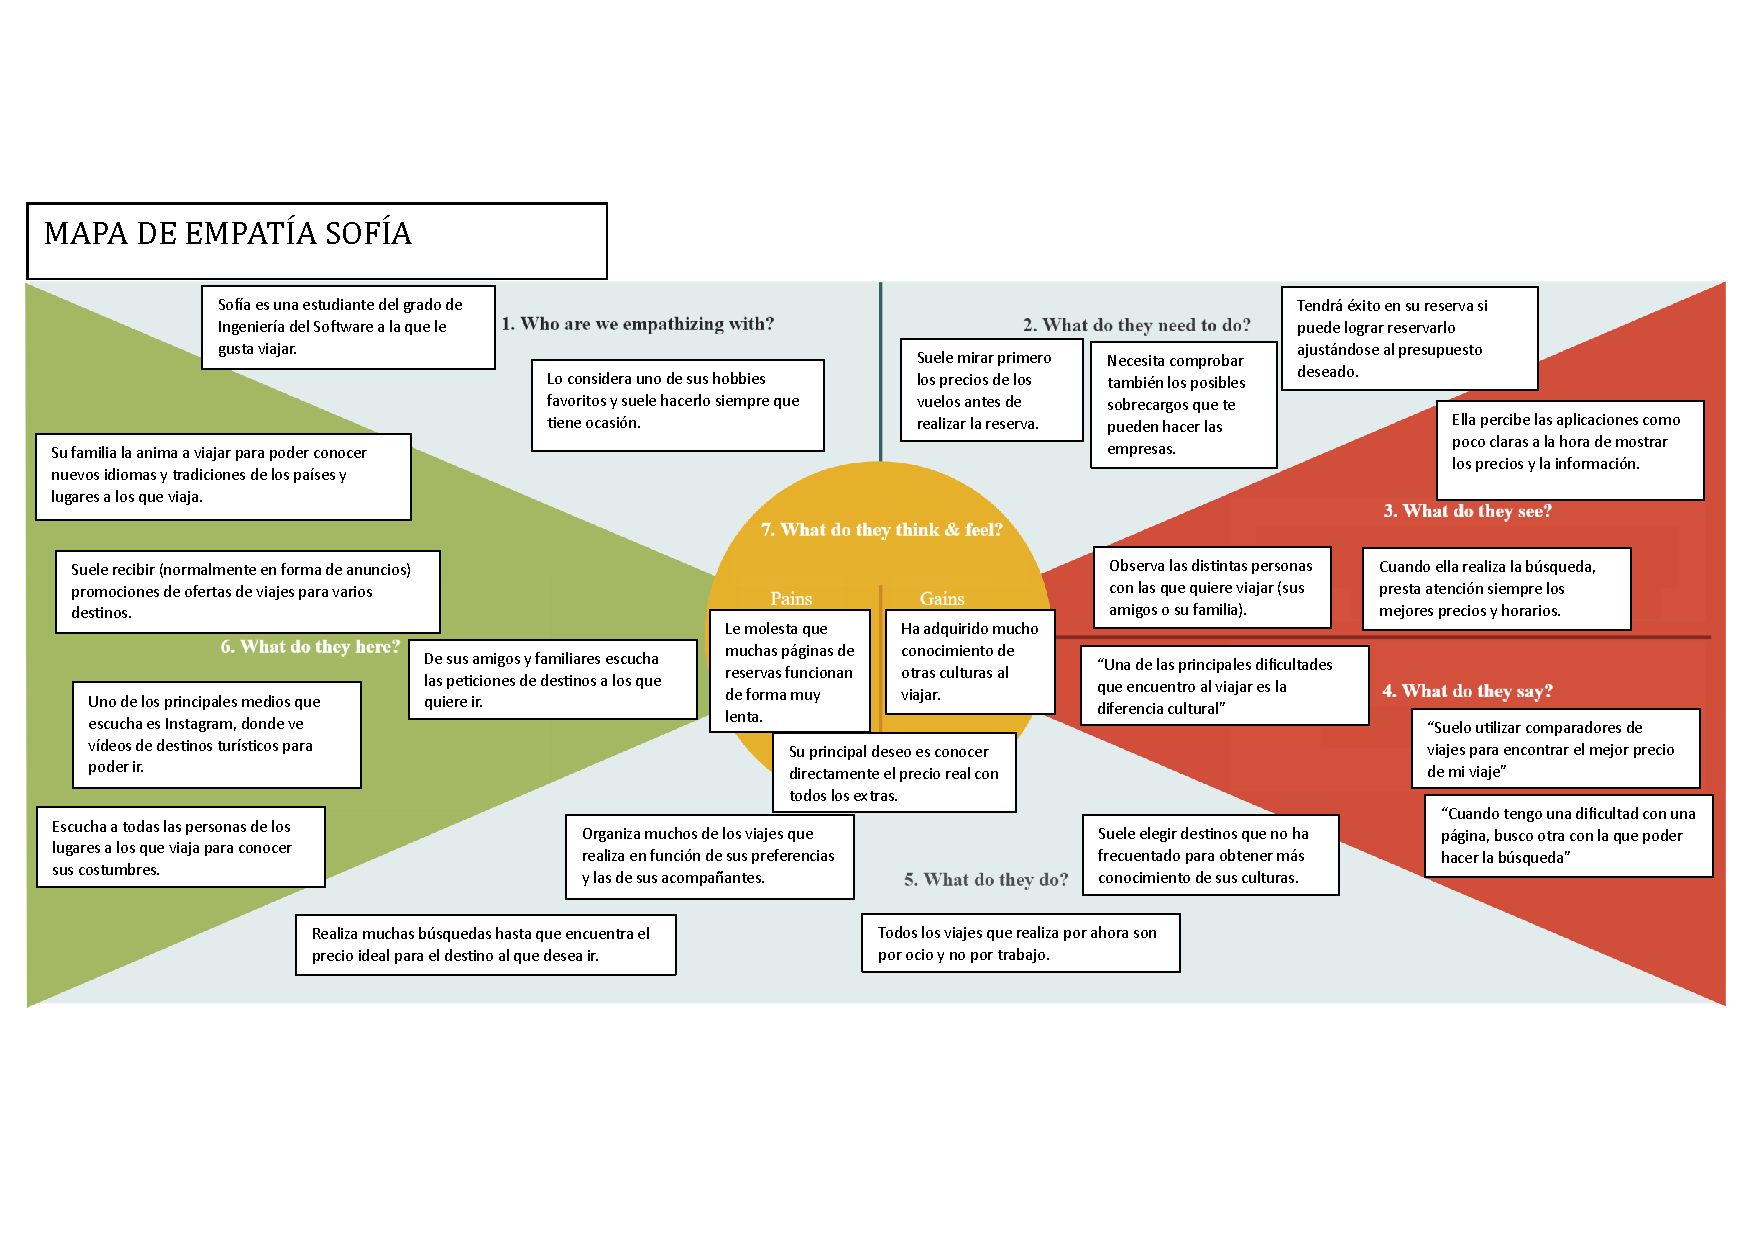
\includegraphics[width=0.9\textwidth]{./mapas_empatia/Mapa de Empatía - Sofía.pdf}
    \caption{Mapa de empatía de la entrevista 2}
    \label{fig:mapa_sofia}
\end{figure}

\begin{figure}[H]
    \centering 
    \includegraphics[width=0.9\textwidth]{./mapas_empatia/Mapa de Empatía - Alberto.pdf}
    \caption{Mapa de empatía de la entrevista 3}
    \label{fig:mapa_alberto}
\end{figure}

\begin{figure}[H]
    \centering 
    \includegraphics[width=0.9\textwidth]{./mapas_empatia/Mapa de Empatía - Beatriz.pdf}
    \caption{Mapa de empatía de la entrevista 1}
    \label{fig:mapa_bea}
\end{figure}

\section{Listado de factoides}

Tras realizar toda la investigación anterior, presentamos los factoides que hemos sacado de cada parte:

\textbf{Factoides de Madi:}

\begin{itemize}
    \item Madi es secretaria de la FEDDI y lleva 16 años trabajando allí.
    \item Madi se encarga de organizar los viajes cuadrando horarios y comprando billetes.
    \item Madi compra billetes a través de Renfe, Air Europa o Iberia porque le sale más económico que en un comparador.
    \item Madi se encarga de los viajes de campeonatos internacionales que les recepciona, les recoge y les lleva al punto de encuentro. Los nacionales los llevan los clubes.
    \item Madi ve que el problema principal para los deportistas es la dependencia de sus padres y entrenadores, el manejo de las aplicaciones y el internet y para algunos necesitan acompañante.
    \item Madi considera que necesitan acompañantes porque tienen problemas para orientarse y no se manejan bien.
    \item Para Madi las dificultades dependen mucho del grado de discapacidad.
    \item Madi no usa aplicaciones, sólo compra en páginas oficiales de la aerolínea.
    \item Madi utiliza la agencia de viajes Betravel para vuelos internacionales.
    \item Madi descarta Ryanair.
    \item Madi no utiliza comparadores porque ya tiene localizadas dos compañías y Renfe que ofrecen el servicio de acompañamiento de Aena.
    \item Madi tiene en cuenta el precio y la variedad de horarios para coger un billete.
    \item Madi no se fija en más facilidades, esos son los atletas.
    \item Madi considera que el comparador debe ser muy simple (lugar, destino y fecha).
    \item A Madi le parece importante que se pueda ver qué tipos de servicios de acompañantes ofrecen.
\end{itemize}


\textbf{Factoides de Sofia:}

\begin{itemize}
    \item Sofía tiene 21 años.
    \item A Sofía le gusta viajar y desde pequeña ha querido conocer las diferentes partes del mundo.
    \item Sofía viaja a menudo, tanto fuera como dentro de España.
    \item A Sofía le encantaría poder viajar más.
    \item Sofía usa tanto automóviles como coches, trenes y autobuses en sus viajes dependiendo del sitio al que viaje.
    \item Sofía prefiere usar autobuses solo cuando viaje distancias cortas o medias.
    \item Sofía ha hecho viajes de varios tipos. Desde intercambios lingüísticos a viajes familiares o con amigos, para conocer nuevas ciudades o relajarse.
    \item A Sofía le gusta ir alternando entre viajar sola, con familia o con amigos, disfruta de todas.
    \item Sofía no recuerda haber tenido ningún problema viajando, aunque admite que cuando viaja lo hace con la mente más abierta de lo que la tiene normalmente.
    \item Sofía a veces organiza los viajes que hace y a veces no.
    \item Sofía busca viajes económicamente accesibles.
    \item Sofía utiliza varios comparadores de viajes a la hora de organizar un viaje. Por ejemplo: Kayak, Skyscanner, Trivago.
    \item A Sofía le gustaría que los comparadores de viajes mostraran el precio final del billete, con los posibles extras incluidos, piensa que es un punto a mejorar.
    \item Sofía prefiere usar aplicaciones web a aplicaciones móviles, y suele hacer estas gestiones desde el ordenador.
    \item Sofía piensa que algunos comparadores son tediosos a la hora de usar, ya que algunos tardan mucho en cargar o te redirigen a otras páginas.
    \item Cuando le ha ocurrido esto, Sofía ha optado por usar otro comparador que no tuviera estos problemas.
    \item Como aportación, a Sofía le gustaría que los comparadores incluyeran el precio final de los billetes, desglosados con los diferentes conceptos.
    \item Sofía considera que los comparadores de viajes son bastante accesibles, pero que quizás aclarar algunas cosas en las webs o los anuncios de spam en las webs pueden molestar a personas con discapacidad intelectual.
    \item Sofía considera que Whatsapp es una aplicación accesible.
\end{itemize}


\textbf{Factoides de Alberto:}

\begin{itemize}
    \item Alberto tiene 22 años y es informático.
    \item Alberto no tiene discapacidad.
    \item Alberto se desenvuelve bien con las tecnologías y le parecen fáciles de usar.
    \item A Alberto le gusta viajar para descubrir historias, paisajes y nuevas culturas.
    \item Alberto viaja exclusivamente por ocio.
    \item Alberto viaja una vez al mes.
    \item A Alberto le gustaría viajar más, más adelante fuera de España.
    \item Alberto usa normalmente vehículo propio para viajar.
    \item Alberto hace 7 años que no viaja en avión.
    \item Alberto usa ocasionalmente taxis, pero prefiere el transporte público.
    \item Alberto descarta el uso de Uber.
    \item Alberto suele viajar con su pareja.
    \item Alberto prepara o busca un itinerario antes de viajar, incluso toma apuntes de paradas por si le falla el móvil o gps, le parece tedioso igualmente y se encarga con su pareja.
    \item Alberto sólo usa comparadores para alojamientos mirando lo visual que sea, la localización y el precio.
    \item Alberto usa Booking y le parece incómodo que le obliguen a poner fechas para ver el precio, prefiere ver el precio directamente.
    \item A Alberto le gusta ver pocas ofertas y más relevantes, y no ver muchas ofertas.
\end{itemize}


\textbf{Factoides de Beatriz:}

\textbf{Factoides del cuestionario:}

\begin{itemize}
    \item La mitad de los usuarios tienen entre 19 y 25 años y la otra mitad entre 26 y 65 años.
    \item La mayoría de los encuestados viven en la ciudad, pocos en pueblos.
    \item Dos tercios de los encuestados tienen un poder adquisitivo medio. Un tercio, bajo y muy pocos, alto.
    \item La mayoría de los encuestados les gusta viajar, pocos no.
    \item La mayoría de los encuestados le gusta viajar por conocer nuevos lugares y los pocos que no, es por la gente o por no parar de moverse.
    \item La mayoría de los encuestados viajan al menos una vez al año, el resto viajan al menos una vez al mes y muy poco no viajan.
    \item La mayoría de los encuestados le gustaría viajar más, el resto no.
    \item Todos los encuestados disfrutan cuando viajan.
    \item Los medios de transporte que usan los encuestados son coche propio, transporte público y aéreo.
    \item Los encuestados suelen viajar por ocio, pocos por trabajo.
    \item Las herramientas que más utilizan los encuestados son Trivago, Kayak y SkyScanner. Hay un tercio de los encuestados que no usan ninguna.
    \item Los comparadores de viajes (Trivago, Kayak, Rastreator, SkyScanner, Momondo) son de fácil uso.
    \item Un quinto de los encuestados tienen alguna discapacidad reconocida.
    \item Los encuestados con discapacidad la mayoría tienen discapacidad física y el resto es intelectual o mental.
    \item Los encuestados con discapacidad dos tercios necesitan adaptaciones para sus viajes como para sillas de ruedas.
    \item La mayoría de los encuestados con discapacidad a veces planifican y el resto o nunca o siempre.
    \item Un tercio de los encuestados con discapacidad encuentran dificultad en el proceso de búsqueda por la accesibilidad.
    \item La mayoría de los encuestados con discapacidad no les supone una dificultad buscar medio de transporte, hacer, comparar y ver las ventajas/desventajas de las rutas o comparar precios.
    \item La mitad de los encuestados con discapacidad no usan comparadores de viajes o similares.
    \item Los encuestados con discapacidad que han usado comparadores la mayoría ha desistido.
    \item Para los encuestados con discapacidad les parece complejo solicitar ayuda dentro de la aplicación de viajes.
    \item La inmensa mayoría de los encuestados sin discapacidad ha viajado en el último año.
    \item La mayoría de los encuestados sin discapacidad hace búsqueda de viaje.
    \item Dos tercio de los encuestados sin discapacidad han utilizado un comparador de viajes.
    \item El motivo principal de los encuestados sin discapacidad es ahorrar dinero. También está mayor oferta, facilidad de uso y ahorra tiempo.
    \item Los encuestados sin discapacidad no tienen problemas con los comparadores.
    \item A los encuestados sin discapacidad les supone una dificultad en el tema de la accesibilidad tener que hacer muchas operaciones para llegar a un objetivo.
    \item Los encuestados están de acuerdo en su mayoría de que está bien la accesibilidad salvo por la ausencia de ayudas al rellenar.
    \item La mayoría de los encuestados no ha echado en falta ninguna funcionalidad.
\end{itemize}


\textbf{Factoides del análisis de competencia}

\section{Modelado}
La fase de modelado es la segunda etapa del proceso de Diseño Guiado por Objetivos (DGO). En esta fase, partiremos de la lista de factoides que
obtuvimos en la etapa anterior y con ella diseñar los prototipos de personas que serán los potenciales usuarios de la misma, representando además
las principales características que extrajimos de los factoides.

Para poder lograr este objetivo, vamos a utilizar el proceso de diseño de personas bottom-up propuesto por Copper, que consta de las siguientes fases:
\begin{itemize}
    \item \textbf{Identificación de variables de comportamiento} $\rightarrow$ El primer paso que vamos a seguir es identificar las distintas variables de comportamiento que vamos a tener en la lista de factoides y ver los posibles valores que van a tomar.
    \item \textbf{Relación de individuos con las variables de comportamiento} $\rightarrow$ Tras haber identificado las variables, vamos a ver para cada uno de los usuarios entrevistados el valor que van a tomar cada una de ellas en base a los factoides obtenidos.
    \item \textbf{Identificación de patrones de comportamiento} $\rightarrow$ Una vez configurada la metriz que relaciona los usuarios con las variables, vamos a marcar en ella las posibles repeticiones que aparezcan para poder establecer un listado de patrones de comportamiento con los que vamos a realizar los esqueletos de las personas.
    \item \textbf{Creación de esqueletos} $\rightarrow$ Tras haber identificado los distintos patrones de comportamiento, vamos a crear los esqueletos que nos van a servir de plantilla para las personas definitivas que vamos a desarrollar en los siguientes apartados.
    \item \textbf{Revisión de la completitud y la redundancia} $\rightarrow$ Cuando los esqueletos de las personas ya estén finalizados, el siguiente paso es comprobar su completitud y evitar posibles redundancias entre ellos, haciendo que todas las personas que se representen tengan todos los factoides y se eviten repeticiones entre ellas.
    \item \textbf{Elaboración de las personas} $\rightarrow$ Al finalizar la revisión de los esqueletos, lo siguiente que ha de hacerse es desarrollar las personas a partir de ellos, dando los principales motivos y acciones que llevan a cada una de ellas.
    \item \textbf{Validación de las personas} $\rightarrow$ Para poder validar las personas, tenemos que cerciorarnos de que representen todos y cada uno de los factoides que tenemos, tanto los de las entrevistas como los de los cuestionarios y el análisis de la competencia.
    \item \textbf{Tipos de las personas} $\rightarrow$ Por último, cuando ya se tienen validadas todas las personas elaboradas, vamos a decir en base a las características que presentan, el tipo de persona ante el que nos encontramos.
\end{itemize}

\subsection{Planificación del hito}
Para poder planificar este hito correctamente, hemos identificado en una Hoja de cálculo (ver figura \ref{fig:planif-hito2}) las distintas tareas que tenemos que 
realizar, junto al intervalo de fechas en el que se encuentra prevista su realización y el / los responsables de dicha tarea.

\begin{figure}[H]
    \centering 
    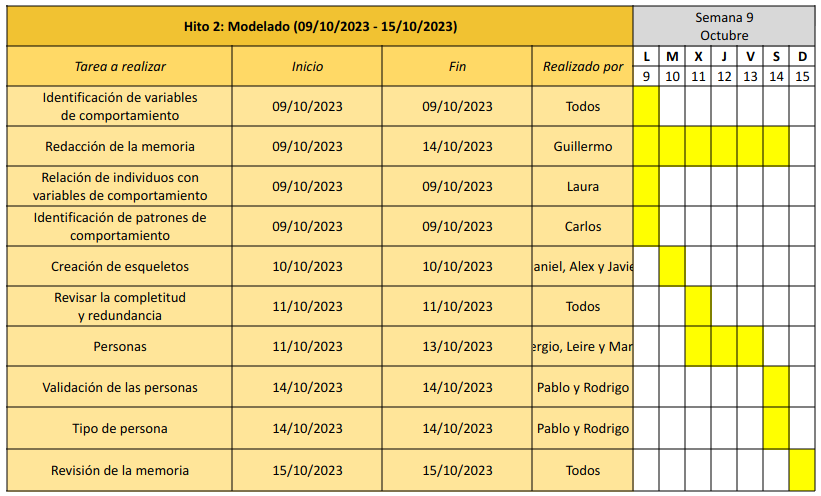
\includegraphics[width=0.5\textwidth]{./Imagenes/Planificaciones/Planif-hito2.png}
    \caption{Planificación Hito 2}
    \label{fig:planif-hito2}
\end{figure}

Dentro de esta planificación, tuvimos varios imprevistos que no contemplamos, como la revisión y corrección de algunas partes del Hito 1 y su posterior incorporación a este hito. Para ello, en primer lugar finalizamos la planificación estipulada de este hito y luego pasamos a realizar la corrección del Hito 1, de modo que sea posible incorporar estos cambios a la nueva lista de factoides para posteriormente volcarlos en las personas.
\subsection{Identificación de variables de comportamiento}
En la fase de modelado, el primer paso que debemos seguir es la identificación de las variables de comportamiento. Estas variables van a ser producto de las listas de factoides que confeccionamos durante el hito anterior y hemos corregido antes de comenzar a trabajar en este. El proceso de confección de las variables consiste en identificar posibles características que pueden encasillar a los usuarios y a partir de ellas darles un rango de valores que podamos asignar a nuestros usuarios. Para reflejar estas variables, hemos construido una tabla (ver cuadro \ref{table:variables-comportamiento}) en la que podemos observarlas junto a los valores que pueden tomar.
\begin{table}[h]
    \centering
    \begin{tabular}{|c|c|}
        \hline
        \textbf{Variable} & \textbf{Posibles valores} \\ \hline
        Rango de Edad & 18- / 18 - 25 / 26 - 40 / 40 - 65 / 65+ \\ \hline
        Estado civil & Casad@ / En pareja / Solter@ \\ \hline
        Organización de viajes & Sí / No \\ \hline
        Uso de comparadores de viajes & Sí / No (Si los usa especificar cuáles) \\ \hline
        Frecuencia de viaje & Baja / Media / Alta \\ \hline
        Tipo de viaje & Ocio / Trabajo / Estudios \\ \hline
        Discapacidad & Sí / No / Acompañante \\ \hline
        Acompañante & Familia / Amigos / Pareja / Solo \\ \hline
        Medio de transporte más frecuente & Avión / Tren / Vehículo propio / Transporte público / Otro \\ \hline
        Uso de tecnología & Básica / Avanzada \\ \hline
        Viaje nacional & Sí / No \\ \hline
        Viaje internacional & Sí / No \\ \hline
        Trabaja & Sí / No \\ \hline
        Gusto por viajar & Sí / No \\ \hline
        Nivel de ahorro & Bajo / Medio / Alto \\ \hline
    \end{tabular}
    \caption{Variables de comportamiento y sus valores}
    \label{table:variables-comportamiento}
\end{table}
\subsection{Relación de individuos con variables de comportamiento}
Tras haber identificado las variables de comportamiento en la fase anterior, vamos a ver para cada uno de los usuarios entrevistados (en base a los factoides
que tenemos registrados) los valores que van a tomar en cada una de ellas. Para mostrar estos resultados vamos a realizar una matriz (ver cuadro \ref{table:relacion-individuos-variables})
en la que vamos a enfrentar cada una de las variables con los entrevistados, poniendo en cada celda el valor que va a tomar la variable para dicho usuario.
\begin{table}[H]
    \centering
    \begin{tabular}{|p{10em}|p{7em}|p{7em}|p{7em}|p{8em}|}
        \hline
        \cellcolor{black}                 & \cellcolor{black}{\textcolor{white}{Madi}}  & \cellcolor{black}{\textcolor{white}{Sofía}}   & \cellcolor{black}{\textcolor{white}{Beatriz}} \\ \hline
        Rango de edad                     &                                             & 18 - 25                                       & 18 - 25                                       \\ \hline
        Estado civil                      &                                             & Soltera                                       & En pareja                                     \\ \hline
        Organización de viajes            & Si                                          & Si                                            & Si                                            \\ \hline
        Uso de comparadores de viajes     & No                                          & Kayak, Skyscanner, Trivago                    & eDreams, comparador de Google                 \\ \hline
        Frecuencia de viaje               & Alta                                        & Media                                         & Baja                                          \\ \hline
        Tipo de viaje                     & Trabajo                                     & Ocio                                          & Ocio                                          \\ \hline
        Discapacidad                      & No                                          & No                                            & No                                            \\ \hline
        Acompañante                       &                                             & Familia                                       & Familia                                       \\ \hline
        Medio de transporte más frecuente &                                             & Transporte público                            & Vehículo propio                               \\ \hline
        Uso de tecnología                 &                                             & Alto                                          & Alto                                          \\ \hline
        Viaje nacional                    & Si                                          & Si                                            & Si                                            \\ \hline
        Viaje internacional               & Si                                          & Si                                            & Si                                            \\ \hline
        Trabaja                           & Si                                          & No                                            & No                                            \\ \hline
        Gusto por viajar                  &                                             & Si                                            & Si                                            \\ \hline
        Nivel de ahorro                   & Alto                                        & Alto                                          & Alto                                          \\ \hline
    \end{tabular}
    \caption{Matriz de relación de los individuos con las variables de comportamiento}
    \label{table:relacion-individuos-variables}
\end{table}

Una vez construida la matriz que relaciona los individuos con las variables, vamos a justificar las razones por las cuáles hemos asignado un
determinado valor a las variables para cada uno de los usuarios. \\

\noindent Justificación de las variables de Madi:
\begin{itemize}
    \item \textbf{Rango de edad} $\rightarrow$ No lo ha comentado.
    \item \textbf{Estado civil} $\rightarrow$ No lo ha comentado.
    \item \textbf{Organización de viajes} (Si) $\rightarrow$ “Madi se encarga de organizar los viajes cuadrando horarios y comprando billetes.”
    \item \textbf{Uso de comparadores de viajes} (No) $\rightarrow$ “Madi no utiliza comparadores porque ya tiene localizadas dos compañías y Renfe que ofrecen el servicio de acompañamiento de AENA.”
    \item \textbf{Frecuencia de viaje} (Alta) $\rightarrow$ “Madi se encarga de los viajes de campeonatos internacionales que ella les recepciona, les recoge y les lleva al punto de encuentro. Madi comenta que hay bastantes campeonatos.” Porque al menos asiste a los viajes internacionales que pueden ser no muy frecuentes.
    \item \textbf{Tipo de viaje} (Trabajo) $\rightarrow$ Se encarga de los viajes de su trabajo y viaja por ello.
    \item \textbf{Discapacidad} (No) $\rightarrow$ Se deduce porque trabaja en una federación y organiza viajes para gente con discapacidad.
    \item \textbf{Acompañante} $\rightarrow$ No lo ha comentado, podría ser sus compañeros de trabajo.
    \item \textbf{Medio de transporte más frecuente} $\rightarrow$ no se sabe realmente, podría ser avión o tren.
    \item \textbf{Uso de la tecnología} $\rightarrow$ tampoco lo comenta, sólo el de los deportistas.
    \item \textbf{Viaje Nacional} (Si) $\rightarrow$ “Madi comenta que en los campeonatos de españa, los clubes son los encargados del desplazamiento de los deportistas, ella interviene poco o nada.” eso significa que el poco puede llegar a viajar en algún momento en los nacionales.
    \item \textbf{Viaje internacional} (Si) $\rightarrow$ “Madi se encarga de los viajes de campeonatos internacionales que ella les recepciona, les recoge y les lleva al punto de encuentro. Madi comenta que hay bastantes campeonatos.”, recoge a los deportistas por lo que hace el viaje.
    \item \textbf{Trabaja} (Si) $\rightarrow$ “Madi es secretaria de la FEDDI y lleva 16 años trabajando allí.”
    \item \textbf{Gusto por viajar} $\rightarrow$ No lo ha dicho.
    \item \textbf{Nivel de Ahorro} (Alto) $\rightarrow$ “Madi compra billetes a través de Renfe, Air Europa o Iberia porque le sale más económico que en un comparador.” suponemos que escoge lo más económico para ahorrar lo máximo posible.
\end{itemize}

\noindent Justificación de las variables de Sofía:
\begin{itemize}
    \item \textbf{Rango de edad} (18 - 25) $\rightarrow$ “Sofía tiene 21 años.”
    \item \textbf{Estado civil} (Soltero) $\rightarrow$ No lo ha comentado, pero parece no tener pareja. 
    \item \textbf{Organización de viajes} (Si) $\rightarrow$ “Sofía a veces organiza los viajes que hace y a veces no.”
    \item \textbf{Uso de comparadores de viajes} (Kayak, Skyscanner, Trivago) $\rightarrow$ “Sofía utiliza varios comparadores de viajes a la hora de organizar un viaje. Por ejemplo: Kayak, Skyscanner, Trivago.”
    \item \textbf{Frecuencia de viaje} (Media) $\rightarrow$ “Sofía viaja a menudo, tanto fuera como dentro de España.”, a menudo será lo normal.
    \item \textbf{Tipo de viaje} (Ocio) $\rightarrow$ “Sofía ha hecho viajes de varios tipos. Desde intercambios lingüísticos a viajes familiares o con amigos, para conocer nuevas ciudades o relajarse.”
    \item \textbf{Discapacidad} (No) $\rightarrow$ “Sofía considera que los comparadores de viajes son bastante accesibles, pero que quizás aclarar algunas cosas en las webs o los anuncios de spam en las webs pueden molestar a personas con discapacidad intelectual.” da a intuir que ella no tiene discapacidad.
    \item \textbf{Acompañante} (Familia) $\rightarrow$ “A Sofía le gusta ir alternando entre viajar sola, con familia o con amigos, disfruta de todas.” Más con familia ya que es estudiante y no tiene trabajo para pagar tantos viajes.
    \item \textbf{Medio de transporte más frecuente} (Transporte público) $\rightarrow$ “Sofía usa tanto automóviles como trenes y autobuses en sus viajes dependiendo del sitio al que viaje.” “Sofía prefiere usar autobuses solo cuando viaje distancias cortas o medias” En cualquiera de los dos casos incluye transporte público.
    \item \textbf{Uso de la tecnología} (Alto) $\rightarrow$ “Sofía tiene 21 años y considera que tiene un buen manejo de la tecnología”
    \item \textbf{Viaje Nacional} (Si) $\rightarrow$ “Sofía viaja a menudo, tanto fuera como dentro de España.”
    \item \textbf{Viaje internacional} (Si) $\rightarrow$ “Sofía viaja a menudo, tanto fuera como dentro de España.”
    \item \textbf{Trabaja} (No) $\rightarrow$ “Sofía es estudiante, tiene 21 años y considera que tiene un buen manejo de la tecnología” 
    \item \textbf{Gusto por viajar} (Si) $\rightarrow$ “A Sofía le gusta viajar y desde pequeña ha querido conocer las diferentes partes del mundo.”
    \item \textbf{Nivel de Ahorro} (Alto) $\rightarrow$ “Sofía busca viajes económicamente accesibles.” quiere ahorrar lo máximo posible.
\end{itemize}

\noindent Justificación de las variables de Beatriz:
\begin{itemize}
    \item \textbf{Rango de edad} (18 - 25) $\rightarrow$ “Beatriz tiene 21 años.”
    \item \textbf{Estado civil} (En pareja) $\rightarrow$ "Va a viajar a ver a su pareja en los próximos meses".
    \item \textbf{Organización de viajes} (Si) $\rightarrow$ “Cuando no viaja con su familia, Beatriz suele organizar los viajes que hace. Cuando va con su familia, lo organiza todo el núcleo familiar en conjunto”.
    \item \textbf{Uso de comparadores de viajes} (eDreams, comparador de Google)
    \item \textbf{Frecuencia de viaje} (Baja) $\rightarrow$ “Beatriz viaja una vez al año, sobre todo dentro de España, y fuera de España una vez cada dos años.” es poco
    \item \textbf{Tipo de viaje} (Ocio) $\rightarrow$ “Beatriz suele viajar para visitar a familiares o por razones de ocio.”
    \item \textbf{Discapacidad} $\rightarrow$ No lo dice en ningún momento.
    \item \textbf{Acompañante} (Familia) $\rightarrow$ “Beatriz suele viajar acompañada, mayoritariamente por algún familiar suyo”.
    \item \textbf{Medio de transporte más frecuente} (Vehículo propio) $\rightarrow$ “Suele viajar en coche o en avión para distancias más largas.” como es dentro de España lo más normal, viaja en vehículo propio más frecuentemente.
    \item \textbf{Uso de la tecnología} (Alto) $\rightarrow$ “Beatriz se desenvuelve bien con las tecnologías y declara usarlas a diario.”
    \item \textbf{Viaje Nacional} (Si) $\rightarrow$ “Beatriz viaja una vez al año, sobre todo dentro de España, y fuera de España una vez cada dos años.”
    \item \textbf{Viaje internacional} (Si) $\rightarrow$ “Beatriz viaja una vez al año, sobre todo dentro de España, y fuera de España una vez cada dos años.”
    \item \textbf{Trabaja} $\rightarrow$ No lo comenta
    \item \textbf{Gusto por viajar} (Si) $\rightarrow$ “A Beatriz le gusta viajar para conocer otros lugares y culturas.”
    \item \textbf{Nivel de Ahorro} (Alto) $\rightarrow$ “Para Beatriz no es ningún problema sacrificar algunas facilidades como el  tipo y la cantidad de equipaje que se puede llevar, el hecho de elegir asiento o los horarios de ida y vuelta porque cuanto más barato mejor.”
\end{itemize}

\subsection{Identificación de patrones de comportamiento}
Para identificar los patrones de comportamiento nos hemos basado en la comparación de los usuarios y buscar similitudes en sus gustos a raíz de las variables de comportamiento previamente estudiadas (ver cuadro \ref{table:relacion-individuos-variables-patrones}).
\begin{table}[H]
    \centering
    \begin{tabular}{|p{10em}|p{7em}|p{7em}|p{7em}|p{8em}|}
        \cellcolor{black}                 & \cellcolor{black}{\textcolor{white}{Madi}}  & \cellcolor{black}{\textcolor{white}{Sofía}}   & \cellcolor{black}{\textcolor{white}{Beatriz}}     \\ \hline
        Rango de edad                     &                                             & \cellcolor{green}{18 - 25}                    & \cellcolor{green}{18 - 25}                        \\ \hline
        Estado civil                      &                                             & Soltera                                       & En pareja                                         \\ \hline
        Organización de viajes            & Si                                          & \cellcolor{green}{Si}                         & \cellcolor{green}{Si}                             \\ \hline
        Uso de comparadores de viajes     & \cellcolor{yellow}{No}                      & \cellcolor{purple}{Kayak, Skyscanner, Trivago}& \cellcolor{purple}{eDreams, comparador de Google} \\ \hline
        Frecuencia de viaje               & \cellcolor{yellow}{Alta}                    & \cellcolor{purple}{Media}                     & \cellcolor{purple}{Baja}                          \\ \hline
        Tipo de viaje                     & Trabajo                                     & \cellcolor{green}{Ocio}                       & \cellcolor{green}{Ocio}                           \\ \hline
        Discapacidad                      & No                                          & \cellcolor{green}{No}                         &                                                   \\ \hline
        Acompañante                       &                                             & \cellcolor{blue}{Familia}                     & \cellcolor{blue}{Familia}                         \\ \hline
        Medio de transporte más frecuente &                                             & Transporte público                            & Vehículo propio                                   \\ \hline
        Uso de tecnología                 &                                             & \cellcolor{green}{Alto}                       & \cellcolor{green}{Alto}                           \\ \hline
        Viaje nacional                    & \cellcolor{orange}{Si}                      & \cellcolor{orange}{Si}                        & \cellcolor{orange}{Si}                            \\ \hline
        Viaje internacional               & \cellcolor{orange}{Si}                      & \cellcolor{orange}{Si}                        & \cellcolor{orange}{Si}                            \\ \hline
        Trabaja                           & \cellcolor{yellow}{Si}                      & No                                            &                                                   \\ \hline
        Gusto por viajar                  &                                             & \cellcolor{green}{Si}                         & \cellcolor{green}{Si}                             \\ \hline
        Nivel de ahorro                   & Alto                                        & \cellcolor{purple}{Alto}                      & \cellcolor{purple}{Alto}                          \\ \hline
    \end{tabular}
    \caption{Matriz de la relación de los individuos con las variables de comportamiento (patrones)}
    \label{table:relacion-individuos-variables-patrones}
\end{table}
Tras realizar el análisis de la matriz anterior hemos identificado los siguientes patrones de comportamiento:
\begin{itemize}
    \item La gente entre 18 y 25 años comparte un gusto por viajar (sobre todo viajes de ocio), tiene un alto uso de la tecnología y tienen un nivel de ahorro alto.
    \item La mitad de las personas utilizan comparadores para organizar los viajes.
    \item La mitad de la gente entrevistada viaja con sus familiares.
    \item A casi todos los entrevistados les gustan los viajes internacionales.
    \item En general la frecuencia de viajes de los usuarios son media-bajas.
    \item Las personas que están solteras viajan con sus familiares.
    \item Las personas que trabajan tienen una frecuencia de viajes alta.
    \item Las personas que no trabajan tienen una frecuencia de viajes media-baja.
    \item Las personas que viajan menos utilizan comparadores de viajes y tienen un nivel de ahorro alto.
    
\end{itemize}

Tras finalizar este proceso de identificación de los patrones de comportamiento, vamos a concluir que tenemos tres tipos de personas. El primero de ellos se trata de personas (normalmente jóvenes) a los que les gusta viajar y se organizan sus propios viajes usando comparadores. El segundo tipo de persona que vamos a tener va a ser personas que tengan un trabajo, que viajan por trabajo y que no organizan sus viajes. Por último, vamos a tener personas con discapacidad (física e intelectual), que desisten al usar los comparadores.

\subsection{Creación de esqueletos}
En el apartado anterior identificamos (de forma descriptiva) los distintos tipos de personas que vamos a tener. El siguiente paso va a ser elaborar el esqueleto de dichas personas, para lo cuál se han seguido los siguientes pasos. En primer lugar se han consultado las distintas listas de factoides y los patrones de comportamiento que se han identificado para ver los tres tipos de usuarios diferenciados que tenemos. Posteriormente se han añadido los factoides identificados en los cuestionarios analizando las estadísticas de estos. A continuación pueden verse los resultados del proceso. \\

\noindent \textbf{Viajante que usa comparadores de viajes}
\begin{itemize}
    \item Marta González Torres
    \item 23 años
    \item Viven en ciudad
    \item Estudiante
    \item Gusto por viajar
    \item Viaja por ocio
    \item Tiene un uso alto de la tecnología.
    \item Tiene una frecuencia de viaje media baja
    \item Persona soltera
    \item Viaja en familia
    \item Utiliza Trivago, SkyScanner, eDreams 
    \item Objetivos:
    \begin{itemize}
        \item Ahorrar la mayor cantidad de dinero posible al realizar el viaje.
        \item Realizar viajes tanto nacionales como internacionales.
    \end{itemize}         
\end{itemize}

\noindent \textbf{Viajante que no usa comparadores de viajes (de forma habitual)}
\begin{itemize}
    \item Juan Martínez Díaz
    \item 24 años
    \item Vive en ciudad
    \item Personas que trabajan
    \item Comparten gusto por viajar
    \item Está en pareja
    \item Viajan por trabajo
    \item Tienen una frecuencia de viaje alta
    \item Tienen un uso alto de la tecnología 
    \item Objetivos:
    \begin{itemize}
        \item Intentar mantener un nivel de ahorro medio.
        \item Poder realizar viajes tanto nacionales como internacionales
    \end{itemize}                      
\end{itemize}

\noindent \textbf{Viajante con discapacidad}
\begin{itemize}
    \item Isabel García Rodríguez
    \item 30 años
    \item Vive en ciudad
    \item Persona con discapacidad física
    \item Planifica sus viajes
    \item Puede encontrar alguna dificultad a la hora de hacer búsquedas (necesita medios accesibles)
    \item Objetivos:
    \begin{itemize}
        \item Poder realizar sus viajes buscando medios de transporte accesibles.
        \item No tiene problemas para comprender la página, pero entiende que hay usuarios a los que sí les puede costar.
        \item Le parece complicado pedir ayuda dentro de los comparadores de viajes.
    \end{itemize}             
\end{itemize}

\subsection{Revisar la completitud y la redundancia}
En esta fase, el objetivo principal es tomar los esqueletos que se han generado en la etapa anterior y comprobar que se encuentran acordes a la lista de factoides y que además no son redundantes entre sí. Para ello, se han comprobado de manera individual los factoides, las variables de comportamiento y los patrones de comportamiento detectados para crear los esqueletos y en cuanto a completitud todo está reflejado en ellos. 
Hay una diferencia clara entre los viajantes que utilizan comparadores y los que no y las personas con discapacidad. 
En cuanto a la redundancia hemos comprobado que no es posible fusionar los esqueletos, ya que, con todas las características presentes, no tienen atributos en común que lo permitan. Por ello, comenzaremos a desarrollar las personas que finalmente van a ser el resultado de este hito.

\subsection{Personas}
Tras haber revisado la completitud y la redundancia de los esqueletos que hemos generado, vamos a elaborar las distintas personas a partir de ellos, garantizando que mantienen todas las características que se han pensado para ellos y que contienen todos los elementos de la lista de factoides. \\

Para configurar estas personas, hemos utilizado un formato en el que vamos a dar en primer lugar la información general de la persona (edad, sexo, estudios y gustos). Posteriormente vamos a poner una foto de la persona (generada por una inteligencia artificial) y por último una descripción más elaborada de la persona, conteniendo la gran mayoría de los factoides e ideas expresadas en los esqueletos de las personas. Para poder destacar estas ideas, las hemos puesto en cursiva. \\

La estructura que van a tener las distintas personas va a tener la siguiente configuración (ver figura \ref{fig:estructura-personas}) con los contenidos que hemos mecionado anteriormente.
\begin{figure}[h]
    \centering
    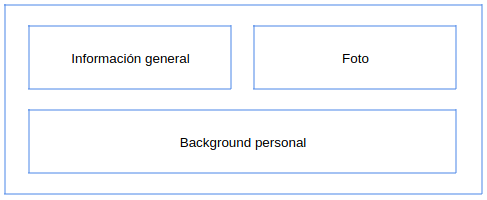
\includegraphics[width=0.5\textwidth]{Imagenes/Personas/Plantilla personas.png}
    \caption{Estructura de las personas}
    \label{fig:estructura-personas}
\end{figure}

\subsubsection{Marta González Torres}

\begin{minipage}{0.4\textwidth}
    \textbf{Información general} \\

    Edad: \textit{23 años} \\
    Sexo: Mujer \\
    Estudios: Ingeniería de Telecomunicaciones \\
    Gustos: Escuchar música e ir a conciertos cuando puede \\
\end{minipage}
\hfill
\begin{minipage}{0.4\textwidth}
    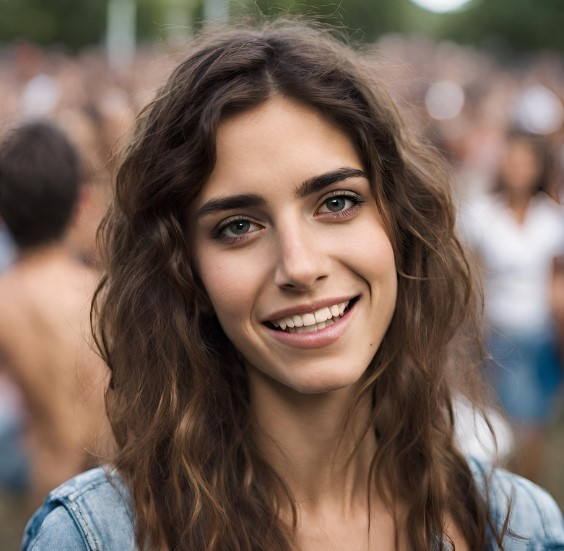
\includegraphics[width=0.5\textwidth]{Imagenes/Personas/Marta.jpg}
\end{minipage}

\textbf{Background personal} \\

Marta no puede salir de su casa sin los auriculares. Para ella la música es una gran parte de su vida, y todas las mañanas, en la parada del bus, \textit{se prepara un playlist personalizada en Spotify} para el itinerario hasta la Universidad. \textit{Vive en Fuenlabrada}, por lo que tiene una ruta de una hora hasta que llega a Madrid, \textit{donde va a clase en la UCM}. \\ 

A Marta sobre todo le gusta la música italiana, ya que en el 2020 se fue de Erasmus a Turín y se enamoró tanto de su cultura como de su música. Su cantante favorita es Francesca Michielin, así que cuando hace gira intenta ir a algún concierto suyo en una \textit{ciudad italiana en la que no haya estado}. \\

Se da la casualidad de que a su hermano Julián también le gusta mucho Francesca, así que en varias ocasiones \textit{han ido ellos de viaje junto a sus padres} Carlos y Elena, los cuáles se van a cenar juntos mientras sus hijos están en el concierto. \textit{Esto no lo hacen muy a menudo} debido a que solo van cuando hay un concierto en alguna ciudad que les resulte interesante a toda la familia. Normalmente se encarga ella de hacer la reserva tanto de los vuelos, \textit{para lo que usa SkyScanner, como del alojamiento, utilizando AirBnB en este caso}. \\

Con respecto al tema universitario, a Marta se le está haciendo cuesta arriba. Se metió inicialmente en telecomunicaciones porque \textit{se le daban bien las matemáticas y la tecnología}, pero la carrera no fue lo esperado. A pesar de las dificultades, la carrera le gusta y querría terminarla, ya que este será en principio su último año. Pero estos problemas la agobian bastante, y para distraerse le gusta mucho \textit{ir a festivales de música por España}. Suele ir todos los años al festival Starlite, pues Pablo, el novio de su hermano y con el que mantiene muy buena relación, es de Marbella, y se puede quedar algunos días en la playa aprovechando el viaje. Pero a pesar de que no tiene que pagar gastos de alojamiento, el evento musical es bastante caro (ya que va varios días), por lo que \textit{intenta ahorrar lo máximo posible en el viaje}. Para eso usa comparadores de viaje como Omio.

\subsubsection{Juan Martínez Díaz}

\begin{minipage}{0.4\textwidth}
    \textbf{Información general} \\

    Edad: \textit{24 años} \\
    Sexo: Hombre \\
    Estudios: Derecho \\
    Gustos: Ir al gimnasio y compartir tiempo con sus amigos. \\
\end{minipage}
\hfill
\begin{minipage}{0.4\textwidth}
    
\includegraphics[width=0.5\textwidth]{Imagenes/Personas/Juan.jpg}
\end{minipage}

\textbf{Background personal} \\

Juan es una persona muy extrovertida y activa, siempre buscando nuevos retos y experiencias. Es por eso por lo que a su temprana edad \textit{ha conseguido un puesto de relevancia en un importante bufete de abogados} y ha conseguido independizarse de sus padres en \textit{un pequeño piso cerca de Moncloa}. \\

Aunque estudió derecho en la Universidad Complutense de Madrid \textit{empezó un curso de programación en Java} ya que le parecía muy interesante aprender y en sus ratos libres realiza pequeños programas que luego prueba y enseña a sus amigos. \\

El bufete en el que trabaja tiene diferentes sedes alrededor del mundo y \textit{de vez en cuando le mandan a comprobar que el trabajo se está realizando correctamente} en cada una, estos viajes les resultan muy cómodos ya que tiene un equipo de personas que le organizan la estancia. \textit{Además de estos viajes, Juan se va de vacaciones cada año fuera de España y cada dos fuera de Europa, le gusta invitar a sus amigos o familia en alguno de los viajes}. \\

Juan conoció a su pareja en el gimnasio de su barrio hace 4 años y desde que están juntos les resulta muy complicado verse entre semana debido a los horarios de ambos. Al año de noviazgo decidieron que para pasar tiempo juntos harían \textit{una escapada cada dos semanas} usando páginas de viajes aleatorios o directamente decirle al hermano de María (su novia) que trabaja en una agencia de viajes, que les organice el viaje.

\subsubsection{Isabel García Rodríguez}
\begin{minipage}{0.4\textwidth}
    \textbf{Información general} \\

    Edad: \textit{30 años} \\
    Sexo: Mujer \\
    Estudios: Psicología \\
    Gustos: Pintura y participar en grupos de apoyo para personas con discapacidad. \\
\end{minipage}
\hfill
\begin{minipage}{0.4\textwidth}
    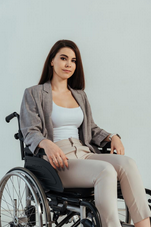
\includegraphics[width=0.5\textwidth]{Imagenes/Personas/Isabel.png}
\end{minipage}

\textbf{Background personal} \\

Isabel es una psicóloga comprometida con la mejora de la calidad de vida de las personas con discapacidad. Tiene una discapacidad física desde su nacimiento que afecta su movilidad y requiere el uso de una silla de ruedas. \\

Ha asistido a varios cursos y conferencias relacionados con la psicología y la discapacidad, lo que la ha llevado a planear viajes a diferentes ciudades para participar en eventos. Utiliza comparadores de viaje para encontrar opciones que se adapten a sus necesidades específicas, como hoteles con habitaciones adaptadas y vuelos con asistencia en el aeropuerto. \\

Aparte de su trabajo, Isabel es una apasionada de la pintura y trata de visitar galerías y estudios de artistas en cada destino que visita. Isabel también es miembro activo de grupos de apoyo para personas con discapacidad en su ciudad, Allí es donde comparte experiencias y ofrece apoyo a otros miembros, por ejemplo a los jóvenes con discapacidad, para fomentar su independencia y autoestima.
Viaja a menudo con su mejor amiga, Carmen, quien la ha apoyado en su viaje de empoderamiento y ha aprendido mucho sobre la discapacidad en el proceso también.

\subsection{Validación de las personas}
Tras revisar las personas obtenidas en el paso anterior, se ha
comprobado que contengan toda la información relevante que sacamos de los factoides,
variables y patrones de comportamiento. También hemos comprobado que todo coincida con los esqueletos de personas. Hemos podido comprobar que en el viajero con discapacidad, en la persona faltaba el factoide de: “Les parece complicado pedir ayuda dentro de las páginas de los comparadores”

Finalmente, el resultado obtenido han sido tres perfiles tal que sus hobbies, background y
objetivos parten de los conocimientos que tenemos acerca de los viajeros que utilizan comparadores, viajeros que no utilizan comparadores, viajeros con discapacidad.

\subsection{Tipos de personas}
\begin{itemize}
    \item \textbf{Persona Primaria} - \textit{Marta González Torres (Viajero que usa comparadores de viajes)} $\rightarrow$ Representa al tipo de usuario consumidor de comparadores de viajes. Se tratan de usuarios que utilizan activamente las funcionalidades de los comparadores con el objetivo de ahorrar lo máximo posible en los transportes para sus viajes.
    \item \textbf{Persona Secundaria} - \textit{Isabel García Rodríguez (Viajero con discapacidad)} $\rightarrow$ Representa al tipo de usuario consumidor o no consumidor de comparadores de viajes que tienen una necesidad añadida o distinta al resto de usuarios. 
    Generalmente usuarios que aparte de la interfaz ya creada necesitaran de una pequeña adaptación visual o sensorial para poder sacar el máximo provecho a la aplicación.
    \item \textbf{Persona Suplementaria} - \textit{Juan Martínez Diaz (Viajero que no usa comparadores de viajes)} $\rightarrow$ Representa al tipo de usuario que no suele usar comparadores de viajes de forma habitual. Buscan experiencias espontáneas y diversas en sus viajes. No es recurrente al uso de comparadores debido a que prefieren contactar con una agencia o familiares que les den todo el trabajo hecho. Pero cuando utilizan los comparadores, las interfaces creadas para satisfacer las necesidades de las personas primarias y secundarias son más que suficientes para satisfacer las suyas.
\end{itemize}

\printglossary[title={Glosario}]

% DESCOMENTAR SI SE USAN IMÁGENES
\let\cleardoublepage\clearpage
\listoffigures
\addcontentsline{toc}{chapter}{Índice de figuras}
\let\cleardoublepage\clearpage

% DESCOMENTAR SI SE USAN TABLAS
\listoftables
\addcontentsline{toc}{chapter}{Índice de cuadros}
\end{document}
